\documentclass[linenumber]{jdsart}

\volume{0}
\issue{0}
\pubyear{2022}
\articletype{research-article}
\doi{0000}

\usepackage{siunitx} % For alignment of numbers
\sisetup{
    group-separator = {,},
    round-mode = places,
    round-precision = 2,
    output-decimal-marker = {.},
    table-number-alignment = center,
    table-figures-integer = 6,
    table-figures-decimal = 2,
    table-figures-uncertainty = 2
}

% image path
\graphicspath{{.}{./images}}

\usepackage{xcolor}
\newcommand{\dt}[1]{\textcolor{purple}{DT: (#1)}}
\newcommand{\jy}[1]{\textcolor{cyan}{JY: (#1)}}

\let\proglang=\textsf
%% \newcommand{\pkg}[1]{{\fontseries{m}\selectfont #1}}
%% \newcommand\code[2][black]{\textcolor{#1}{\texttt{#2}}}

\usepackage{comment}
\usepackage{booktabs, textgreek}

%% float control
\renewcommand\floatpagefraction{0.75}
% \renewcommand\topfraction{.8}
% \renewcommand\bottomfraction{.8}
% \renewcommand\textfraction{.2}
\setcounter{totalnumber}{50}
\setcounter{topnumber}{50}
\setcounter{bottomnumber}{50}

\begin{document}

\begin{frontmatter}
  
\title{Principles for Open Data Curation: A Case Study with the New
York City 311 Service Request Data}
\runtitle{Principles for Open Data Curation}

\author[1]{\inits{D.}\fnms{David}~\snm{Tussey}}
\author[2]{\inits{J.}\fnms{Jun}~\snm{Yan}}
\address[1]{\institution{NYC DoITT}, \cny{USA}}
\address[2]{Department of Statistics,
  \institution{University of Connecticut}, \cny{USA}}



 \tableofcontents % Optional: Table of Contents
 \listoffigures % List of Figures
 \listoftables % List of Tables

\hyphenpenalty=750

\begin{abstract}
In the early 21st century, the open data movement began to transform 
societies and governments by promoting transparency,
innovation, and public engagement. New York City (NYC) has been at
the forefront of this movement since the enactment of the Open 
Data Law in 2012, which led to the creation of the NYC Open Data
portal. This portal now hosts 2,700 datasets from 80 city agencies,
serving as a crucial resource for research across various domains, 
including health, urban development, and transportation. The 
success of these initiatives highlights the importance of data 
curation in ensuring the utility and reliability of open datasets.
This paper examines the challenges of open data curation through a
case study of the NYC 311 Service Request (SR), addressing issues 
of data validity, consistency, and curation efficiency. Based on 
insights from this case study, we propose a set of data curation 
principles tailored for government-released open data. These principles 
aim to enhance data management practices and ensure 
the ongoing utility of open data. The paper concludes with 
actionable recommendations for enhancing data curation and outlines
general principles for the effective release of open data.

\end{abstract}

\begin{keywords}
  \kwd{Data cleansing}
  \kwd{Data Curation}
  \kwd{Data science}
  \kwd{NYC Open Data}
  \kwd{Open data}
  \kwd{Smart Cities}
  \kwd{Transparency}
\end{keywords}

\end{frontmatter}

\section{Introduction} 
\label{sec:intro}

In the early 21st century, the open data movement began 
to take shape, driven by the fundamental belief that 
freely accessible data can transform both societies and 
governments. This movement champions the principles
of transparency, innovation, and public engagement. 
A landmark in this journey was the launch of the United States'
\href{https://www.data.gov}{Data.gov} portal in 2009, a pioneering
platform in making government data widely accessible. Shortly after,
the European Union followed suit, unveiling its
\href{https://data.europa.eu/euodp}{Open Data Portal} in 2012, further
cementing the movement's global reach. Furthermore, the World Bank's Open
Data initiative, initiated in 2010, stands out as a comprehensive
repository for global development data, available at
\href{https://data.worldbank.org}{World Bank Open Data}. 
These initiatives represent significant strides in democratizing data, 
breaking down barriers that once kept valuable information 
on government performance in silos. Their collective impact 
extends beyond mere data sharing to fostering a culture of openness 
that benefits individuals, communities, governments, and economies worldwide 
\citep{barns2016mine, wang2016adoption}.


New York City (NYC) has emerged as a leader in the open data movement,
marked by the enactment of the Open Data Law in 2012
\citep{zuiderwijk2014open}. This landmark legislation led to the
creation of the \href{https://opendata.cityofnewyork.us}{NYC Open Data
  portal}, which today hosts an impressive array of 2,700 datasets
from 80 different city agencies. This resource has become invaluable
for researchers across various fields and has significantly enhanced
local government transparency. Popular datasets include information on
restaurant health inspection violations, car crashes, high school and
college enrollment statistics, jail inmate charges, and the location
of city-wide free Internet access points. These datasets have been
applied in civil life in various ways, such as mapping car crashes
involving pedestrians and visualizing high school and college
enrollment trends. Furthermore, they have enabled significant research
across multiple domains, including health \citep{cantor2018facets,
  shankar2021data}, urban development \citep{neves2020impacts}, and
transportation \citep{gerte2019understanding}, aiding in the
understanding and addressing of complex urban challenges.


Data curation, the process of organizing, maintaining, and ensuring
the quality of datasets, plays a crucial role in maximizing the
utility of open data. Proper curation ensures that datasets remain
consistent, accurate, and useful for diverse applications. For example, 
curating data ensures it can be leveraged effectively for machine learning 
systems, which require high-quality data to produce reliable insights
\citep{polyzotis2019data, jain2020overview}. Poor 
curation may result in issues such as missing data, formatting errors, or 
inconsistent values that can lead to biased or inaccurate outcomes
\citep{geiger2020garbage}.
This is particularly critical in domains where machine learning is applied 
to sensitive tasks, such as public health or policy
\citep{rahm2000data}.


Research into data curation has explored these challenges in depth. 
Among the earliest discussions, \citet{witt2009constructing} focused 
on developing data curation profiles tailored to specific contexts, 
setting a precedent for targeted data management strategies. 
Addressing broader challenges in data sharing and management, 
\citet{borgman2012conundrum} highlighted the complexities of 
research data distribution, emphasizing the need for robust 
strategies. This is complemented by \citet{hart2016ten}, who outlined 
essential principles for effective data management, particularly 
emphasizing meticulous curation practices. The utility of curated 
open data is vividly illustrated in public health and global challenges, 
where \citet{cantor2018facets} demonstrated the utility of curated 
data in evaluating community health determinants, and 
\citet{shankar2021data} observed its critical role during the 
COVID-19 pandemic in managing collective responses.


The contributions of this paper are twofold. First, we delve into
the specifics of data curation challenges using the NYC 311 Service
Request (SR) Data as a case study. This dataset serves as a prime 
example for examining key issues in data curation, including data 
validity, consistency, and curation efficiency. 
We illustrate these points with live examples drawn from our 
processing of the 311 SR data. Secondly, building upon insights 
gained from this case study, we propose a set of data curation 
principles tailored for government-released open data. These 
principles are designed to address the unique challenges 
and requirements observed in the curation of such datasets.


The paper is organized as follows. Section~\ref{sec:data} provides 
an overview of the history of the NYC 311 SR system and presents 
a summary of SR counts over the 10-year period from 2014 to 2023. 
Section~\ref{sec:issues} delves into specific data cleansing 
challenges affecting data quality and curation efficiency, 
including structural problems, adherence to the data dictionary, 
and the presence of missing, blank, or N/A entries. This section 
also investigates field compliance with legal or acceptable values, 
highlights logical inconsistencies, and examines concerning patterns 
in the data. We explore the balance between precision and accuracy 
and identify duplicate or redundant fields, along with observations 
on the Data Dictionary. Section~\ref{sec:recommendations} offers 
practical recommendations for mitigating or resolving these issues, 
while Section~\ref{sec:discussion} encapsulates key insights and 
discusses the broader implications of our findings.


\section{NYC 311 SR Data} 
\label{sec:data}
The NYC 311 service, a critical component of New York City's public
engagement and service response framework, serves as a centralized hub
for non-emergency inquiries and requests. Introduced in 2003, the NYC
311 system was designed to streamline the city's response to
non-emergency issues, ranging from noise complaints to street
maintenance requests. Initially a phone-based call center, the system
evolved into a comprehensive data management platform handling
millions of requests annually. Key milestones since its launch in 2003
include the addition of online and mobile app channels in 2009, a
\jy{should we mention the system upgrade just before the pandemic to
  document this historical event?}
record high of 348,463 monthly service requests in August 2020 due to
the COVID-19 pandemic, the 2021 expansion to include the MTA's city
subway system, and a record 3.23 million service requests in
2023. Today, the NYC 311 data system manages over 3 million service
requests per year. This data is publicly accessible through the NYC Open Data
Portal, which provides tools for querying, grouping, aggregating,
geo-mapping, visualizing, and exporting results. The
\href{https://www.nyc.gov/content/oti/pages/}{NYC Office of Technology
  and Innovation (OTI)}, which provides technological support for the
open data system. 

\begin{comment}
Despite its success, the 311 system faces several challenges:
data timeliness, accuracy, and consistency, difficulties in
correlating data over long periods, excluding personally
identifiable information (PII), integration with stand-alone systems
at selected NYC agencies, and managing API usagefor numerous
third-party users. These challenges are addressed by various agency
open data managers and 
\end{comment}

The impact of NYC 311 data extends beyond operational efficiency; it
has become instrumental in shaping city governance and community
engagement. This open data not only ensures governmental transparency
but also empowers researchers, civic developers, and the general
public. The data has been pivotal in providing advice on shelters
during emergencies, handling inquiries during the COVID-19 pandemic,
enforcing standards between landlords and tenants, reallocating taxi
routes based on analyses by the Taxi and Limousine Commission (TLC),
and improving responsiveness across City Agencies


\begin{figure}[tbp]
	\centering
  	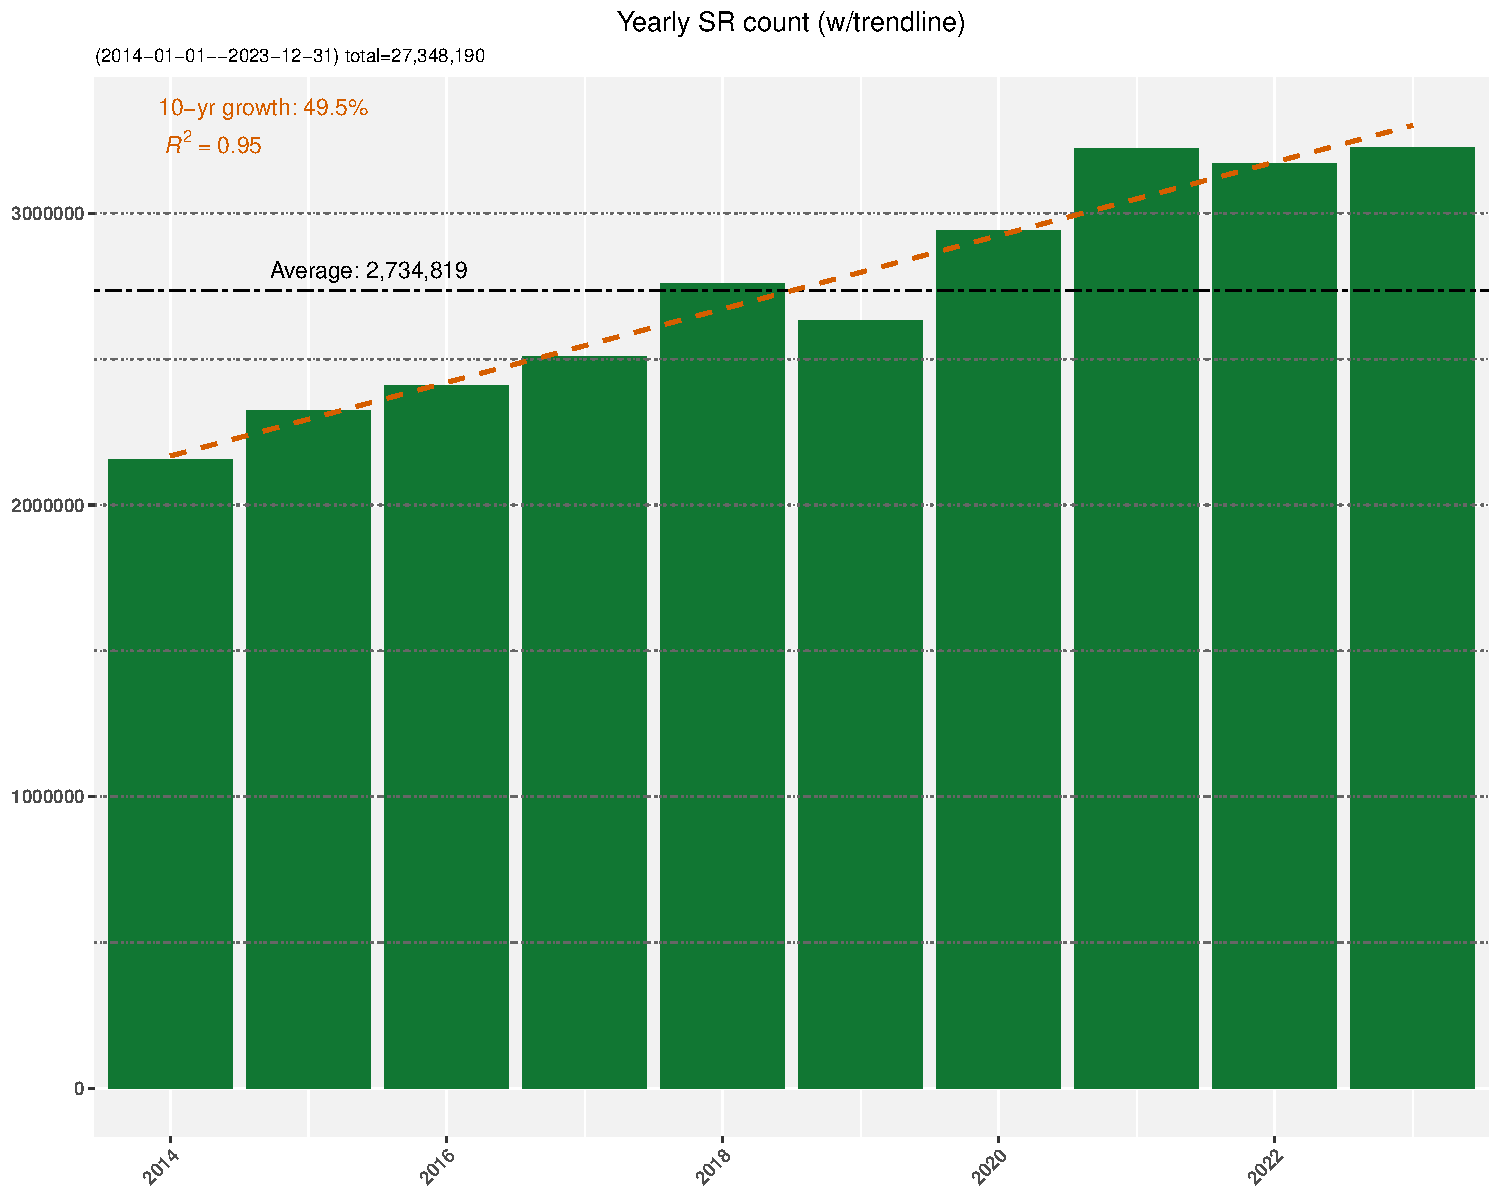
\includegraphics[width=0.7\textwidth]{10-year-trend_yearly.pdf}
 	\caption{10-year (2014-2023) annual SR Counts.}
  	\label{fig:10-yr}
\end{figure}


Our investigation focused on a 10-year period (2014--2023), downloaded
on \jy{Give date because the data is updated daily.}
This version of the data is available as a supplement to facilitate
reproducibility of the analysis presented in the sequel.
\jy{How many total? file size? Somewhere we used only two years that
  need to be clarified.}
Figure~\ref{fig:10-yr} shows the annual counts of NYC 311 SR over the
10-year period from 2014 to 2023, revealing a clear upward trend in
public engagement with the system. The most significant increase
occurred in 2020, when the number of requests surged to 3.23 million
due to the COVID-19 pandemic, illustrating the essential role of the
311 system in supporting residents during times of crisis. Overall, SR
counts increased by nearly 49.5\% between 2014 and 2023, reflecting
growing public reliance on the system for addressing non-emergency
issues. The steady rise in SRs can be attributed to the increased
accessibility of the 311 system via online and mobile platforms, as
well as heightened public awareness of the service. While the spike in
2020 was exceptional, the broader trend indicates sustained growth in
service request volume over the decade, highlighting the system's
evolving role in managing both routine city operations and
extraordinary events.

\jy{The 'title' in each figure could be removed because we have
  captions. The fonts of the annotations in the figures need to be
  increased. The code generating them need to be tidied for future
  sharing.
}

\jy{The plot sizes seem to be fixed in the generation code. That's why
  the fonts are small when scaled. I'd generate them with approxiately
  the expected sizes in the manuscript. I'd also use aspect ratio
  0.618 (golden ratio).
}

Figure~\ref{fig:SRcountbyAgency} provides a breakdown of SRs by
agency, showing the cumulative percentage of SRs handled by each
agency over a given time period. This figure highlights that the
distribution of SRs is concentrated among a few key agencies. The six
largest agencies are New York Police Department (NYPD), 
Housing Preservation and Development (HPD),
New York City Department of Sanitation (DSNY), Department of
Transportation (DOT), Department of Environmental Protection (DEP),
and Department of Parks and Recreation (DPR).
They collectively handle over 90\% of the total SR volume. This is
indicative of the critical roles these agencies play in managing
public concerns, ranging from noise complaints and housing issues to
sanitation and transportation problems. The NYPD alone accounts for a
substantial portion of the total SRs, underscoring its central role in
addressing complaints related to public safety and order. The
remaining 10\% distributed across a large number of smaller
agencies. This concentration of requests points to the systemic
reliance on a few key departments for resolving most non-emergency
issues, further emphasizing the importance of optimizing data handling
and curation processes within these high-volume agencies to ensure
efficiency and responsiveness.


\begin{figure}[tbp]
	\centering
	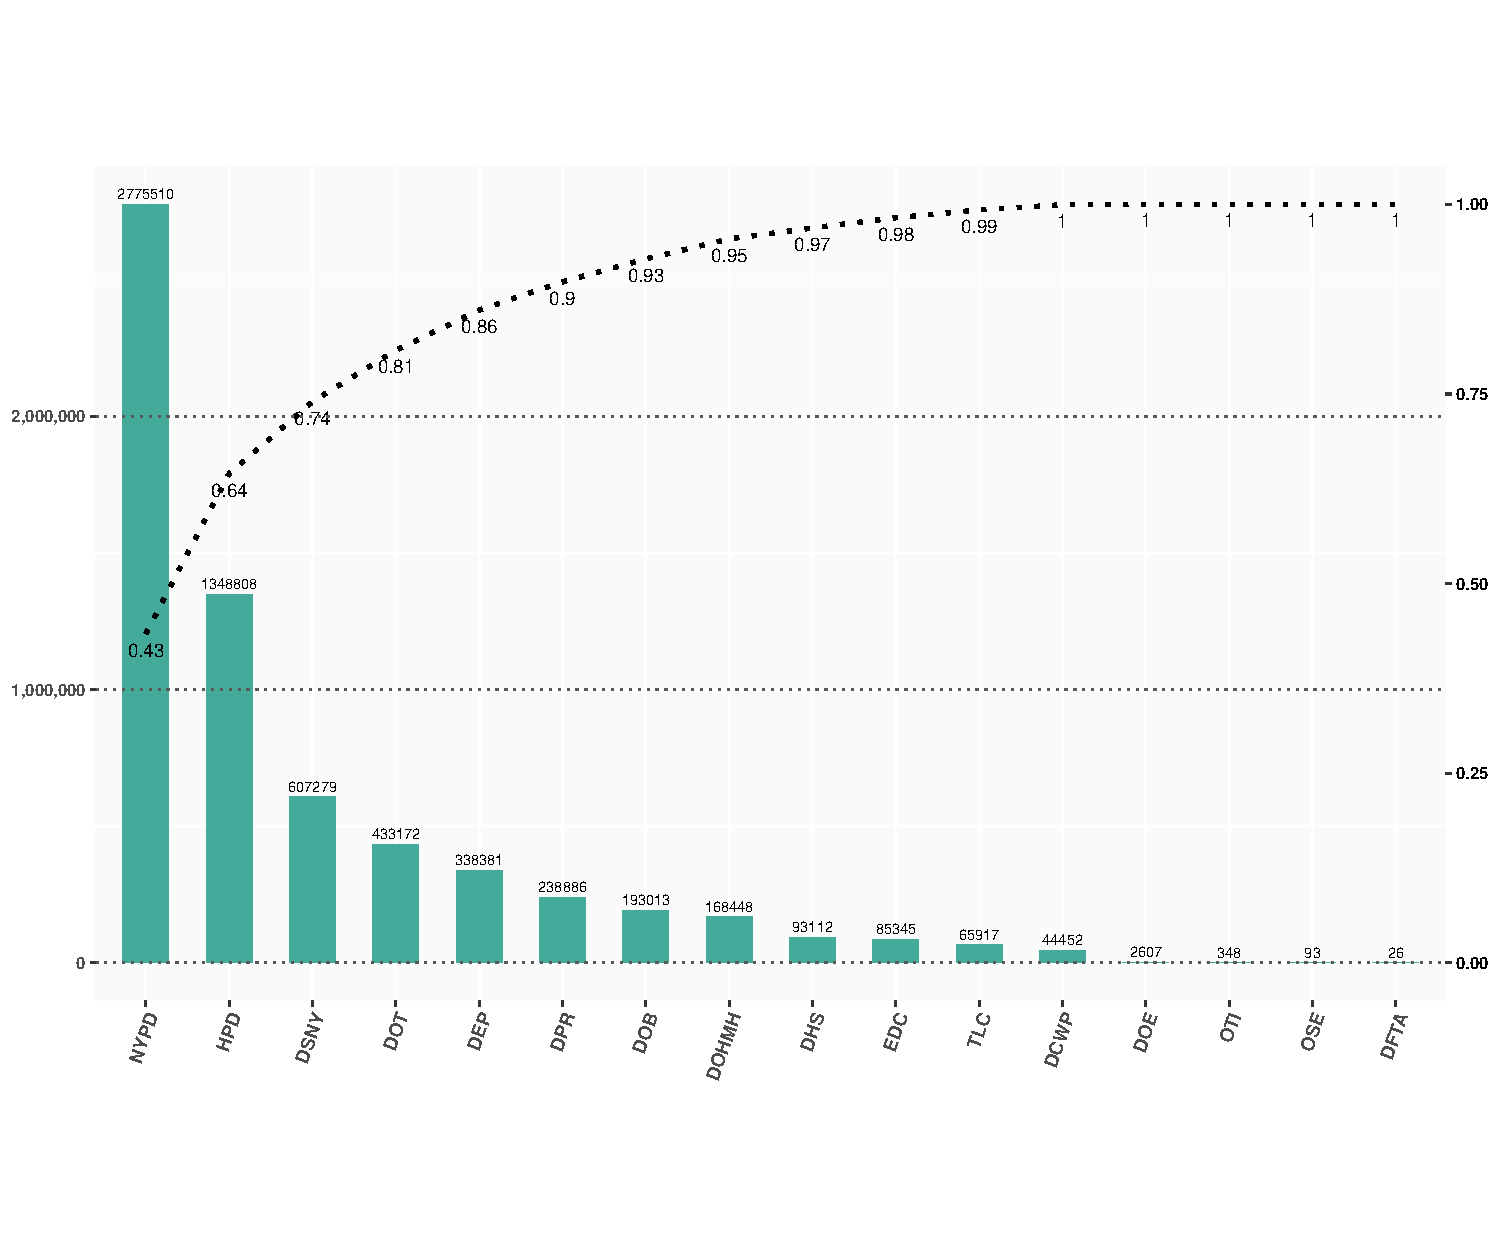
\includegraphics[width=0.7\textwidth]{SRs_by_Agency.pdf}
  	\caption{SR counts by Agency with Cumulative Percentage}
	\label{fig:SRcountbyAgency}
\end{figure}


\begin{comment}
\begin{table}[tbp]
  \centering
  \caption{Noise-related complaints\_type(s) by count with Agency}
  \label{tab:noisecomplaints}
  \begin{tabular}{@{}lS[table-format=7.0,round-mode=places,
    round-precision=0]S[table-format=2.2,round-mode=places,
    round-precision=2]l@{}} % 'l' for left-aligned, 'S' for siunitx number alignment
    \toprule
    \textbf{complaint\_type} & \textbf{Count} & \textbf{Percentage} & \textbf{Agency} \\ 
    \midrule
    Noise - Residential        & 675502 & 10.56 & NYPD  \\ 
    Noise - Street/Sidewalk    & 300507 &  4.70 & NYPD  \\ 
    Noise - Commercial         & 128892 &  2.02 & NYPD  \\ 
    Noise - Vehicle            & 115956 &  1.81 & NYPD  \\ 
    Noise                      & 100413 &  1.57 & DEP   \\ 
    Noise - Helicopter         &  85345 &  1.33 & EDC   \\ 
    Noise - Park               &  16620 &  0.26 & NYPD  \\ 
    Noise - House of Worship &   2757 &  0.04 & NYPD  \\ 
    \bottomrule
  \end{tabular}
\end{table}
\end{comment}



\begin{figure}[tbp]
 \centering
  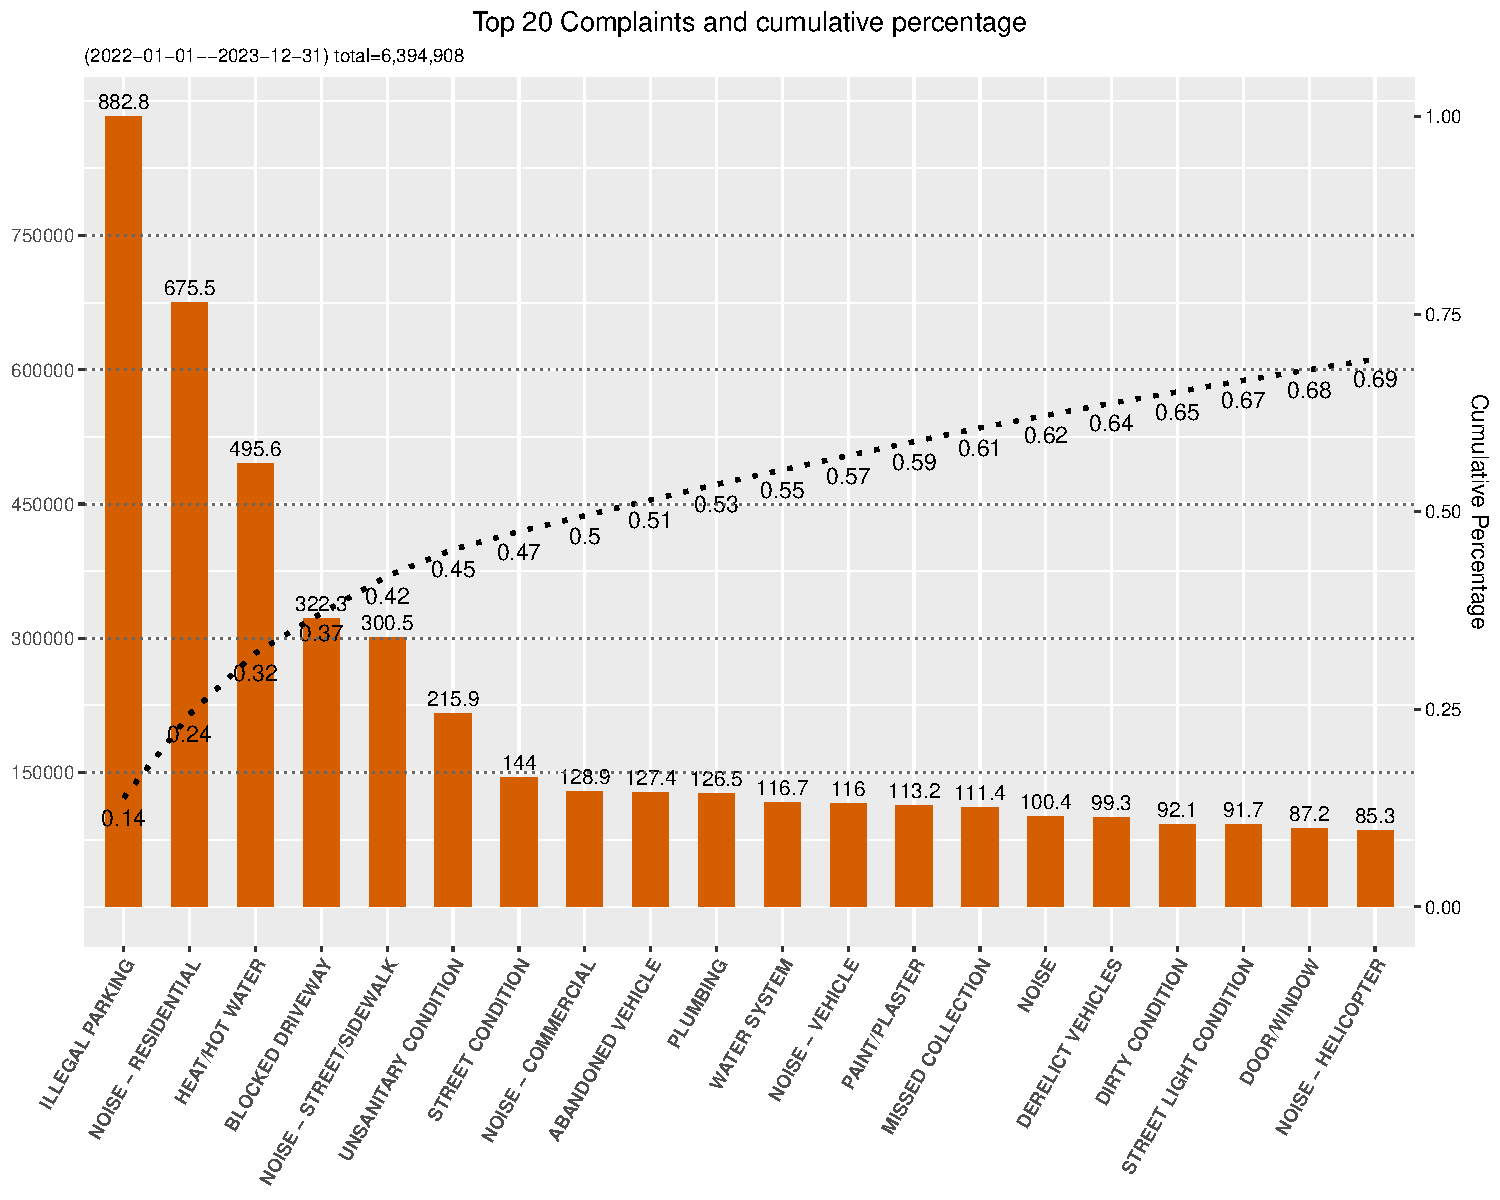
\includegraphics[width=0.7\textwidth]{SR_by_Complaint_Type.pdf} 
  \caption{Top 20 complaint type(s) and Cumulative Percentage} 
  \label{fig:SR_complaints}
\end{figure}

Figure~\ref{fig:SR_complaints}
illustrates the top 20 complaint types, accounting for 70\% 
of all Service Requests (SRs), and their cumulative percentage. The 
distribution of complaints is skewed, with a small number of issues 
dominating the total SR volume. Noise-related complaints, including 
residential, commercial, and street noise, make up 22\% of all 
complaints, making them the most frequent issue in the NYC 311 system. 
Other prominent categories include illegal parking, heat/hot water 
complaints, and blocked driveways. The cumulative percentage curve 
shows that after the top 20, the remaining complaint types are spread 
thinly across the remaining 30\% of SRs. This concentration suggests 
that improving responses to the most frequent complaints could have 
a significant impact on overall service efficiency and resident 
satisfaction. It also provides insights into the operational 
pressures faced by the city agencies responsible for handling these 
high-volume complaints.


\section{NYC 311 SR Data Cleansing Issues} 
\label{sec:issues}

Data cleansing refers to the process of identifying and rectifying
errors, inconsistencies, and inaccuracies within datasets to ensure
they are of high quality and reliable for analysis
\citep{maletic2005data, hosseinzadeh2023data}. The process
typically involves removing duplicate records, handling missing or
incomplete data, correcting mislabeled or inaccurate entries, and
standardizing data formats \citep[e.g.,][]{cody2017cody,
  van2018statistical}. In the context of open data, cleansing is
especially important as open datasets often come from diverse,
uncoordinated sources, leading to variations in data quality,
completeness, and consistency. Without proper cleansing, the utility
of open data can be severely limited, affecting its reliability for
research, policy-making, and innovation. The main purpose of cleansing
open data is to ensure that it is accurate, consistent, and usable
across multiple platforms and by various stakeholders. This improves
the trustworthiness of the data and enables better decision-making,
more accurate analysis, and the integration of data into machine
learning models or other systems.


% What is data cleansing?  Wikipedia 
% \href{https://en.wikipedia.org/wiki/Data_cleansing}{Data Cleansing} 
% offers this definition. 

% \begin{quote}\textit{Data cleansing or data cleaning is the process of detecting and 
% correcting (or removing) corrupt or inaccurate records from a record set, 
% table, or database and refers to identifying incomplete, incorrect, 
% inaccurate or irrelevant parts of the data and then replacing, 
% modifying, or deleting the dirty or coarse data.}
% \end{quote}


Many quality criteria are employed to ensure high-quality data 
processing. One of the primary efforts is data validation, which spans 
several critical checks. For instance, mandatory fields must not be 
left empty, ensuring that key information is always captured. 
Additionally, certain fields must conform to specific data types, 
such as numeric, character, or date formats, which are typically 
outlined in a Data Dictionary. Another essential aspect of validation 
is domain compliance, where fields must adhere to a predefined set of 
values, such as statuses, state names, zip codes, or gender. Structural 
errors also play a significant role in data quality, particularly when 
naming conventions or data entries are inconsistent. Common issues 
include fields that do not appear in the Data Dictionary or the 
inconsistent use of blanks, spaces, NA, N/A, or ``<NA>'' to indicate 
missing data. Furthermore, redundant or irrelevant fields can clutter 
datasets, reducing efficiency. Logical inconsistencies are another 
important consideration, such as related fields that violate expected 
relationships, like a ``due date'' that precedes the ``created date.'' 
Lastly, the balance between accuracy and precision is crucial, as both 
must be carefully managed to ensure reliable and meaningful data.


Here we identify the presence of issues in the NYC 311 SR open data;
not necessarily to solve them. A solution effort should
be undertaken only after an investigation as to the why and how 
such issues came about, and a discussion as to whether or not it 
is an \textit{error}. 


\subsection{Structural Issues}
\label{sec:structural}

Structural issues refers to how data is organized, formatted, 
or presented within a dataset. Structural issues can make 
it difficult to analyze the data effectively. Here are some 
characteristics of the 311 SR data set:

\begin{itemize}
	\item There are 47 columns of data for each row, exportable as a CSV file.
	
	\item There are four date fields (created, closed, updated, due).
	
	\item There are three borough fields; two of which appear to be duplicates.
	
	\item Two zip code fields, but not duplicates
	
	\item Seven street fields; two pair of which appear to be duplicates
	
	\item Two Police Precinct fields; not duplicates
	
	\item In addition to the incident\_address, there are five additional location fields: 
	lat/long, street\_name, landmark, NY State plane, and Block \#
	
	\item One free-form text field, resolution\_description, which 
	supports 934 characters of input, including commas and special characters
\end{itemize}

The 311 SR 
\href{https://data.cityofnewyork.us/api/views/erm2-nwe9/files/b372b884-f86a-453b-ba16-1fe06ce9d212?download=true&filename=311_ServiceRequest_2010-Present_DataDictionary_Updated_2023.xlsx}{Data Dictionary} 
identifies 41 data columns (fields) and provides related information 
for each. However, upon downloading the data, six additional fields 
appear that are not included in the Data Dictionary. These fields are 
visible in the portal's Column Manager widget, labeled with the prefix 
``@computed\_region.'' The additional fields include \texttt{zip\_codes}, 
\texttt{community\_districts}, \texttt{borough\_boundaries}, 
\texttt{city\_council\_districts}, \texttt{police\_precincts}, and 
\texttt{police\_precinct}. While one can infer the meaning and 
derivation of these computed fields to some extent, uncertainty remains. 
The critical question is whether these fields can be reliably used for 
analytical purposes reliable documentation. In particular, which one
of the two percinct fields should one use? What is the difference
between the computed zip codes and the incident zipcode among the 41
documented variables?


\subsection{Missing Data}
\label{sec:blanks}
Understanding the absence of data by field is important 
when undertaking analysis. For example, if you wanted to 
determine if SRs were closed before or after their
\texttt{due\_date}, you would be challenged as 99.6\% of the
\texttt{due\_date} field is
blank. When counting fields for blank or N/A values, they appear 
to divide into three groups:
\textbf{Mostly Empty}, \textbf{Partially Empty}, 
and \textbf{Few/None Empty}. 
The Mostly Empty category ranges from 93--99.9\% blank 
and includes such fields as
\texttt{taxi\_company due\_date},
\texttt{pickup\_location}, and \texttt{landmark}.
The Partially Empty includes such fields as
\texttt{location\_type}, \texttt{borough}, 
and \texttt{cross\_street}. And the Few/None Empty includes
\texttt{created\_date}, \texttt{complaint\_type},
\texttt{agency}, and \texttt{status}. In some cases it may make
sense to inquiry as to why some fields are frequently blank.
Figure~\ref{fig:blank_fields} presents a graphic 
depiction of total empty (blank \& N/As) for each fields illustrating
the grouping into the Most, Partial, and Few categories.

\jy{Can we lighten the color of the bar to make the pertentages more
  legible?}


\begin{figure}[tbp]
	\centering
  	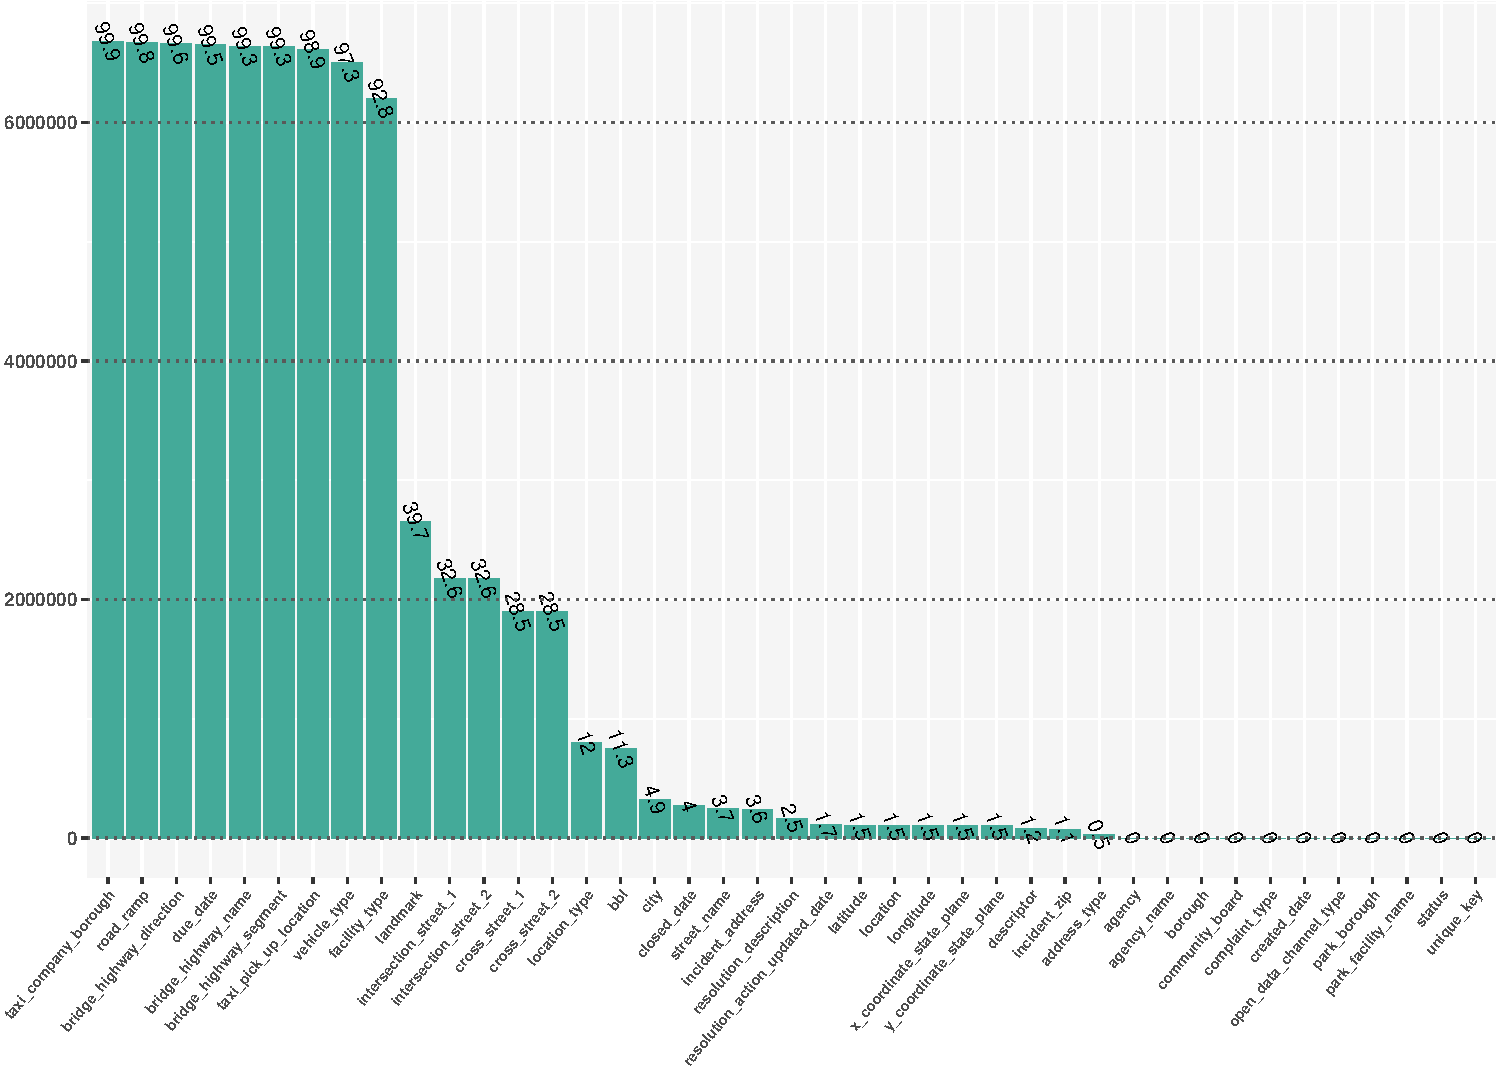
\includegraphics[width=\textwidth]{BlankFields.pdf}
	\caption{Number and Percentage of Empty/Blank Entries}
	\label{fig:blank_fields}
\end{figure}


\subsection{Validating Data for Acceptable Values}
\label{sec:domain}
Any analytic effort must ensure that fields containing invalid values 
are identified and removed from the analysis. Below are the results of 
selected field validation. The latitude and longitude fields were 
found to fall within the geographic boundaries of New York City, and 
the \texttt{unique\_key} field was indeed unique, as required. 
Unfortunately, the Data Dictionary specifies very few domains of 
acceptable values. However, the following fields were tested and found 
to comply with their expected domains, as determined by public usage 
and historical datasets: \texttt{address\_type}, \texttt{status}, 
\texttt{borough}, \texttt{borough\_boundaries}, \texttt{park\_borough}, 
\texttt{data\_channel}, \texttt{vehicle\_type}, and 
\texttt{city\_council\_district}. Some fields proved to be problematic 
as to their compliance with a domain of legal values. 


\paragraph{Zip Codes}
\label{sec:zipcodesissues}
All zip codes (two fields: \texttt{zip\_codes} and \texttt{incident\_zip}) 
should be valid as defined by the USPS database, which contains 
37,946 valid zip codes. However, the computed field \texttt{zip\_codes} 
proved problematic, with over 58\% (3.6 million) of its entries being 
invalid. Although the more accurate \texttt{incident\_zip} field has 
only 0.07\% invalid entries, this still results in 4,163 errors, which 
is not insignificant. The breakdown of invalid entries in the 
\texttt{zip\_codes} field, sorted by Agency, shows that the
\jy{Which agency? Missing a table? We could prepare a supplement where
  we can put additional tables/figures without limit.}
distribution by percentage mirrors the overall breakdown of SRs by 
Agency, potentially indicating a systemic problem.

\begin{table}[tbp]
    \centering
    \caption{Comparison of Top Ten Zip Codes Lists}
	    \begin{tabular}{@{}lS[table-format=6.0,round-mode=places,
	    round-precision=0]c@{\hskip 0.5cm}@{}lS[table-format=6.0,
	    round-mode=places,round-precision=0]c@{}}
		\toprule
	 	\multicolumn{3}{c}{\textbf{zip\_codes}} & \multicolumn{3}{c}{\textbf{incident\_zip}} \\
	      \cmidrule(r){1-3} \cmidrule(l){4-6}
	      \textbf{Zip Code} & \textbf{Count} & \textbf{Valid?} 
	      & \textbf{Zip Code} & \textbf{Count} & \textbf{Valid?} \\
	      \midrule
	        11275 & 104556 & FALSE & 10466 & 104562 & TRUE \\
	        12420 & 27503 & TRUE & 10023 & 27972 & TRUE \\
	        12428 & 26564 & TRUE & 10031 & 25548 & TRUE \\
	        10935 & 25508 & FALSE & 10457 & 25066 & TRUE \\
	        10934 & 23448 & FALSE & 10453 & 24752 & TRUE \\
	        10931 & 22381 & TRUE & 10456 & 24751 & TRUE \\
	        10930 & 22121 & TRUE & 10452 & 22527 & TRUE \\
	        17613 & 21963 & FALSE & 10025 & 21705 & TRUE \\
	        10936 & 21707 & FALSE & 10458 & 21689 & TRUE \\
	        11606 & 21435 & FALSE & 10032 & 20622 & TRUE \\
	      \bottomrule
	    	\end{tabular}
 	\label{tab:zipcodes}
\end{table}

Consider a case study with the NYC Office of Nightlife (ONL). Suppose 
that ONL wants to know, "What are the top 10 zip codes for Noise 
Complaints over the last two years?" ONL seeks to assess the impact 
of recent efforts promoting a vibrant nightlife in NYC while also 
easing tensions between bar and club owners. Assume this analysis uses 
the \texttt{zip\_codes} field, one of the computed fields known to have 
validity issues. The analysis is then repeated using the more accurate 
\texttt{incident\_zip} field. Finally, both analyses are validated 
against the USPS zip code database. The top 10 zip codes and their 
validation results are summarized in Table~\ref{tab:zipcodes}. Six out 
of the ten \texttt{zip\_codes} entries are invalid, closely matching 
the overall dataset's 58\% invalid rate. In contrast, the 
\texttt{incident\_zip} field is fully valid, consistent with the 
overall \texttt{incident\_zip} validation rate of 99\%.
It is possible that the computed \texttt{zip\_codes} may mean the zip
code of something differnent from the incident. Without proper
documentation, it is confusing to have it in the released data.


\paragraph{Police Precincts}
\label{sec:police-precincts}
A curious case arises when examining two nearly identical fields: 
\texttt{police\_precincts} and \texttt{police\_precinct}. Both fields 
are among the computed fields previously mentioned. Using the 
\href{https://www.nyc.gov/site/nypd/bureaus/patrol/precincts-landing.page}
{NYPD Precinct listings}, it is possible to determine the valid police 
precincts. Upon validation, both \texttt{police\_precincts} and 
\texttt{police\_precinct} contain about 35\% invalid entries. However, 
the invalid entries are not identical. The \texttt{police\_precincts} 
field has 2,171,864 invalid entries (35\%), while the 
\texttt{police\_precinct} field has 2,171,778 invalid entries (also 
35\%), but they do not match.



\paragraph{Community Boards}
\label{sec:communityboards}
Community Boards are the most local, grassroots form of City government, 
serving as a vital connection between communities, elected officials, 
and City agencies. They often act as a measure of the equity of City 
services across the five boroughs. In the 2022-2023 dataset, there are 
27,276 invalid \texttt{community\_board} entries, representing 0.43\% 
of non-blank data. The distribution of these invalid entries by Agency 
is not consistent with the overall SR Agency 
distribution. This suggests that issues may exist within specific key 
Agencies, such as the Taxi \& Limousine Commission (TLC) and the 
Department of Parks and Recreation (DPR).


\paragraph{Community Districts}
\label{sec:communitydistrict}
Another of the computed fields is \texttt{community\_districts}. 
Community Districts define the geographic boundaries for the Community 
Boards but differ in that they are used by the Department of City 
Planning (DCP) for environmental, socio-economic, and demographic 
purposes. They represent a geographical division rather than a City 
government division. Due to the format of the \texttt{community\_district} 
data, it is not possible to directly establish validity. However, the 
dataset contains 72 unique entries, while only 59 valid Community 
Districts exist.


\paragraph{Date and Closed Date}
\label{sec:negativeduration}
For the \texttt{created\_date} and \texttt{closed\_date} fields, one 
might expect that these fields are automatically populated by the SR 
application software when setting an SR status to ``new'' or ``closed.'' 
Unfortunately, this does not seem to be the case, as several anomalies 
exist in the date fields:
\begin{itemize}
    \item SRs with a \texttt{closed\_date} that occurs before the 
    \texttt{created\_date}.
    \item \texttt{created\_date(s)} and \texttt{closed\_date(s)} in 
    the far distant past.
    \item \texttt{created\_date(s)} and \texttt{closed\_date(s)} that 
    match to the second.
    \item A large number of SRs closed and/or created exactly at midnight 
    or noon, to the second.
\end{itemize}


\subparagraph{Closed before Created: Negative Duration}
Citizens, NYC Government Officials, and Agencies use the created and 
closed dates to measure the ``duration'' of SRs, which reflects Agency 
responsiveness. While duration is not directly present in the dataset, 
it can be easily computed as the difference between
\texttt{(closed\_date} and \texttt{created\_date}.
There are 12,251 SRs where the \texttt{closed\_date} precedes the 
\texttt{created\_date}, generating nonsensical ``negative durations.'' 
Though this represents only 0.2\% of the dataset, these errors can 
significantly impact response time analyses.
Eight SRs with extremely large negative durations ($-$730 days), all 
originating from the Department of Homeless Services (DHS), contain 
an entry of ``1900-01-01'' as the \texttt{closed\_date}. This results 
in negative durations exceeding $-$44,601 days (or 122 years). Such 
anomalies, though rare, can significantly skew statistical results if 
not addressed during data cleansing. As a result, these SR rows are 
removed from the analysis. 

\begin{table}[tbp]
  \centering
  \caption{Negative duraton of the largest magnitude (days) excluding
    extreme negative values}
  \begin{tabular}{l l l r l}
    \toprule
    {created\_date} & {closed\_date} & {duration} 
    & \textbf{agency} \\
    \midrule
    2023-01-27 14:40:00 & 2022-01-14 14:40:00 & $-$378.0 & DOT \\
    2023-01-18 10:06:00 & 2022-01-12 10:06:00 & $-$371.0 & DOT \\
    2023-01-27 14:36:00 & 2022-01-22 14:35:00 & $-$370.0 & DOT \\
    2023-01-11 11:10:00 & 2022-01-09 11:10:00 & $-$367.0 & DOT \\
    2023-12-18 03:13:00 & 2023-01-16 13:10:00 & $-$335.6 & DOT \\
    \bottomrule
  \end{tabular}
  \label{tab:largest-errors}
\end{table}


\begin{figure}[tbp]
	 \centering
 	 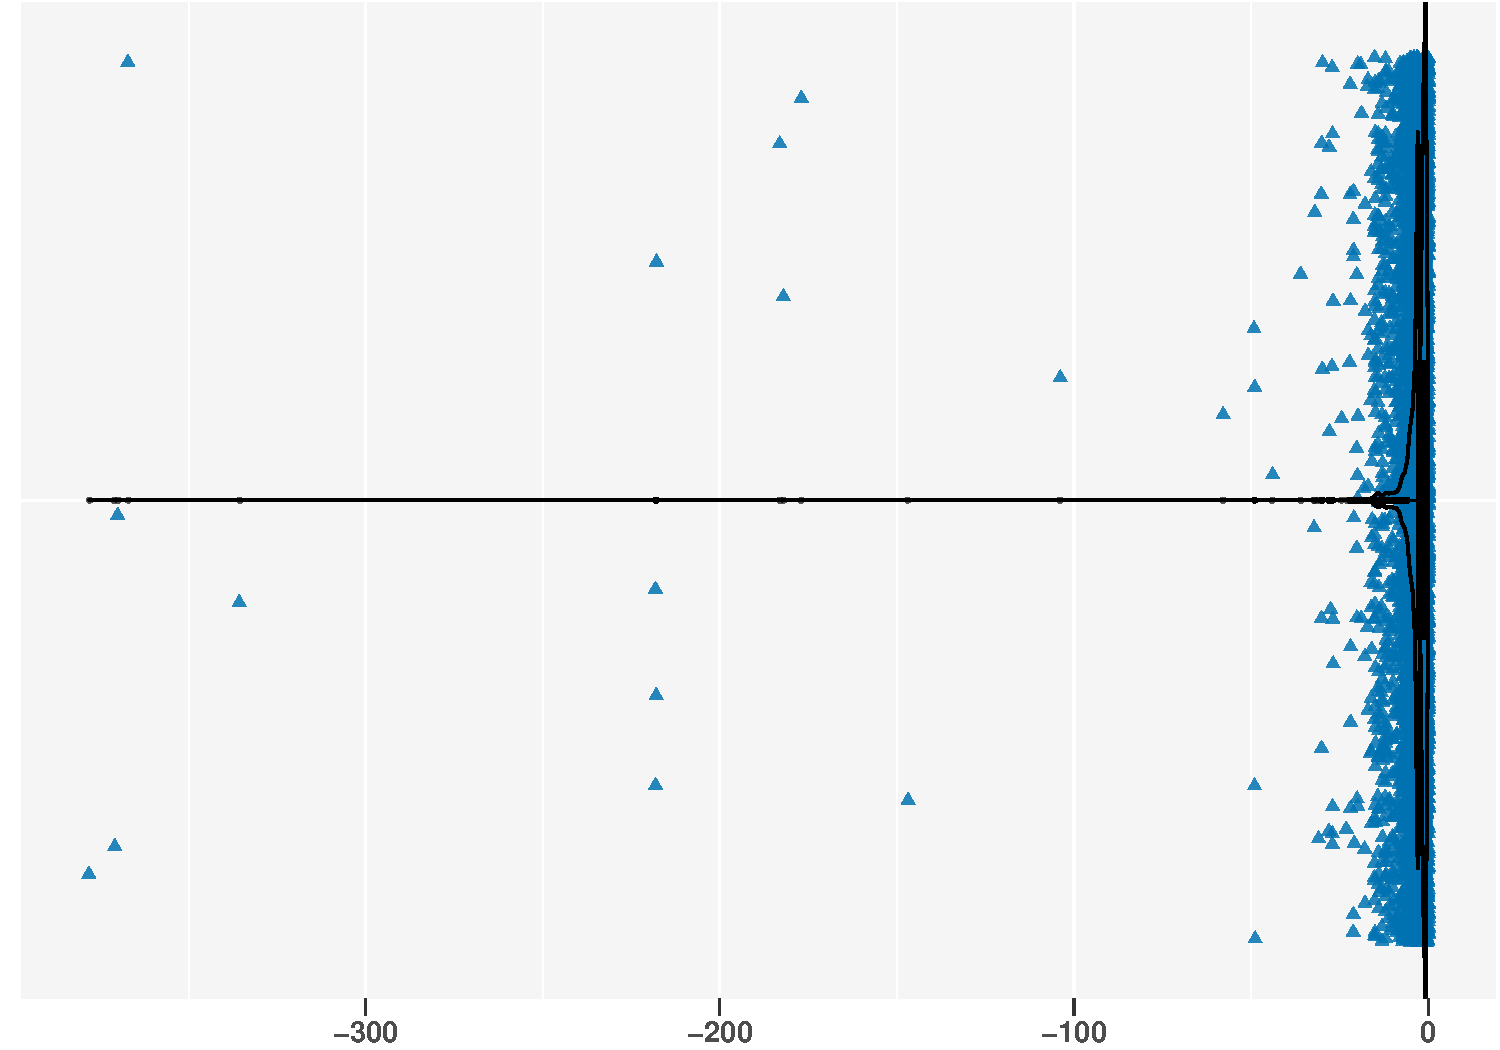
\includegraphics[width = 0.7\textwidth]{negative_duration_SR_violin.pdf}
 \caption{Distribution of Negative Durations}
 \label{fig:negative-duration-violin}
\end{figure}


Excluding the extreme negative values, 
Figure~\ref{fig:negative-duration-violin} shows the broad spread of 
negative-duration SRs. While there are few outliers, the magnitude 
of the negative durations is troubling and can produce bizarre 
analytical results. Table~\ref{tab:largest-errors} summarizes the 
negative durations of the largest magnitude (in days). The data 
suggests that the negative duration issue is predominantly a problem 
within the Department of Transportation (DOT), where 95\% of these 
errors occur.


% For illustration, consider a case study of homeless person
% assistance. Suppose that DHS wants to know ``How 
% quickly have 311 SRs for ``Homeless Person Assistance'' been resolved 
% over the past two years?'' This is a typical request made by 
% both the public and City government; analogous to ``How quickly 
% is my Agency responding to ``critical'' requests, and does 
% that performance vary by Borough, Zip Code, etc. To conduct such an 
% analysis, we can use the tools on the Open Data Portal. Here are the steps:
		
		
% \begin{itemize}
%     \item Select created\_date from 2022-2023 and filter by complaint\_type = 
%     ``Homeless Person Assistance'' (this yields 55,000 SRs)
    
%     \item Compute the ``duration'' (closed\_date – created\_date)
    
%     \item Take an average of the ``duration'' field  which yields: \textbf{Answer:  -4.8 days}  
% \end{itemize}

		
% Clearly that answer is nonsensical. How did such a simple task result 
% in an absurd answer? The answer lies in the computation of the ``duration'' 
% field. It turns out, there are eight DHS SRs that have a closed\_date 
% of ``1900-01-01''. Each of those SRs creates a negative duration of -44,602 
% days (-122 years). Those eight SRs are enough to drive the 
% average duration of 55,000 Homeless Assistance SRs to a negative 
% value; clearly incorrect. In this case, the median is a better measure 
% of central tendency. The median is  0.2 days (approx 5 hrs) which will
% surely please the DHS. 

		
%\begin{figure}[tbp]
% 	 \centering
 %	 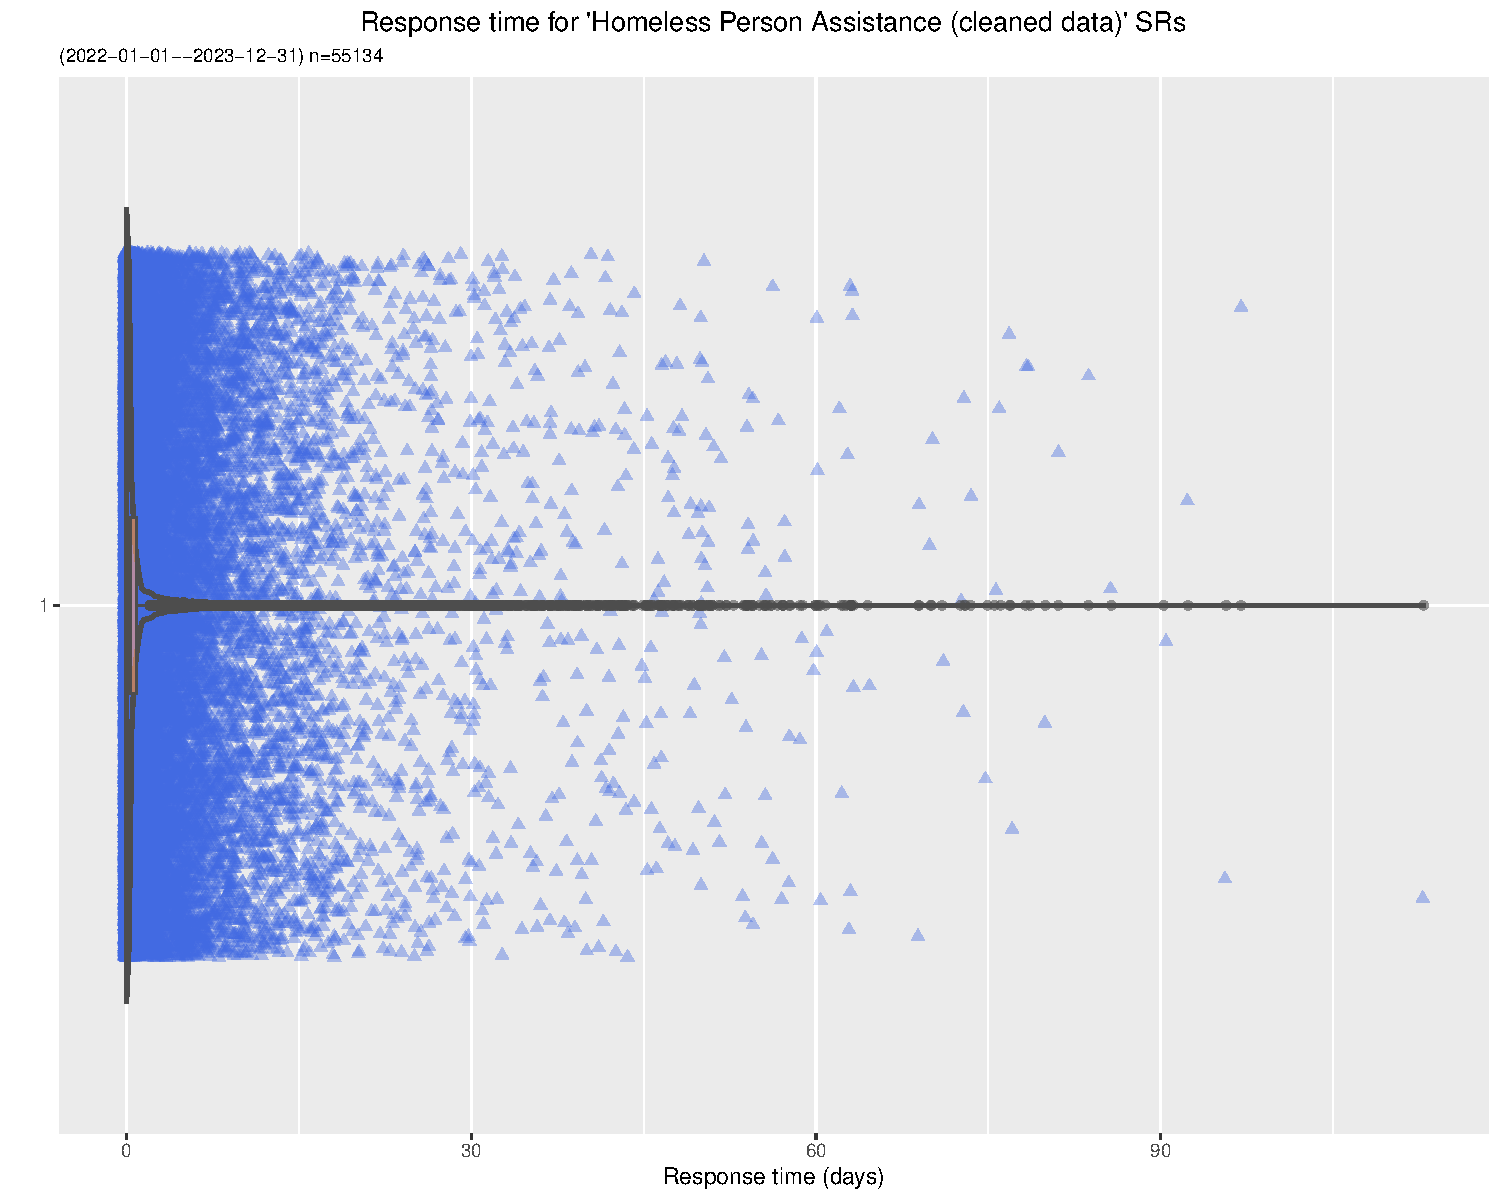
\includegraphics[width = \textwidth]{homeless_response_time_clean.pdf}
%	 \caption{Homeless Assistance SR Durations}
%	 \label{fig:homeless}
%end{figure}

\subparagraph{Resolution Action Update Date}
	
\begin{figure}[tbp]
  \centering
  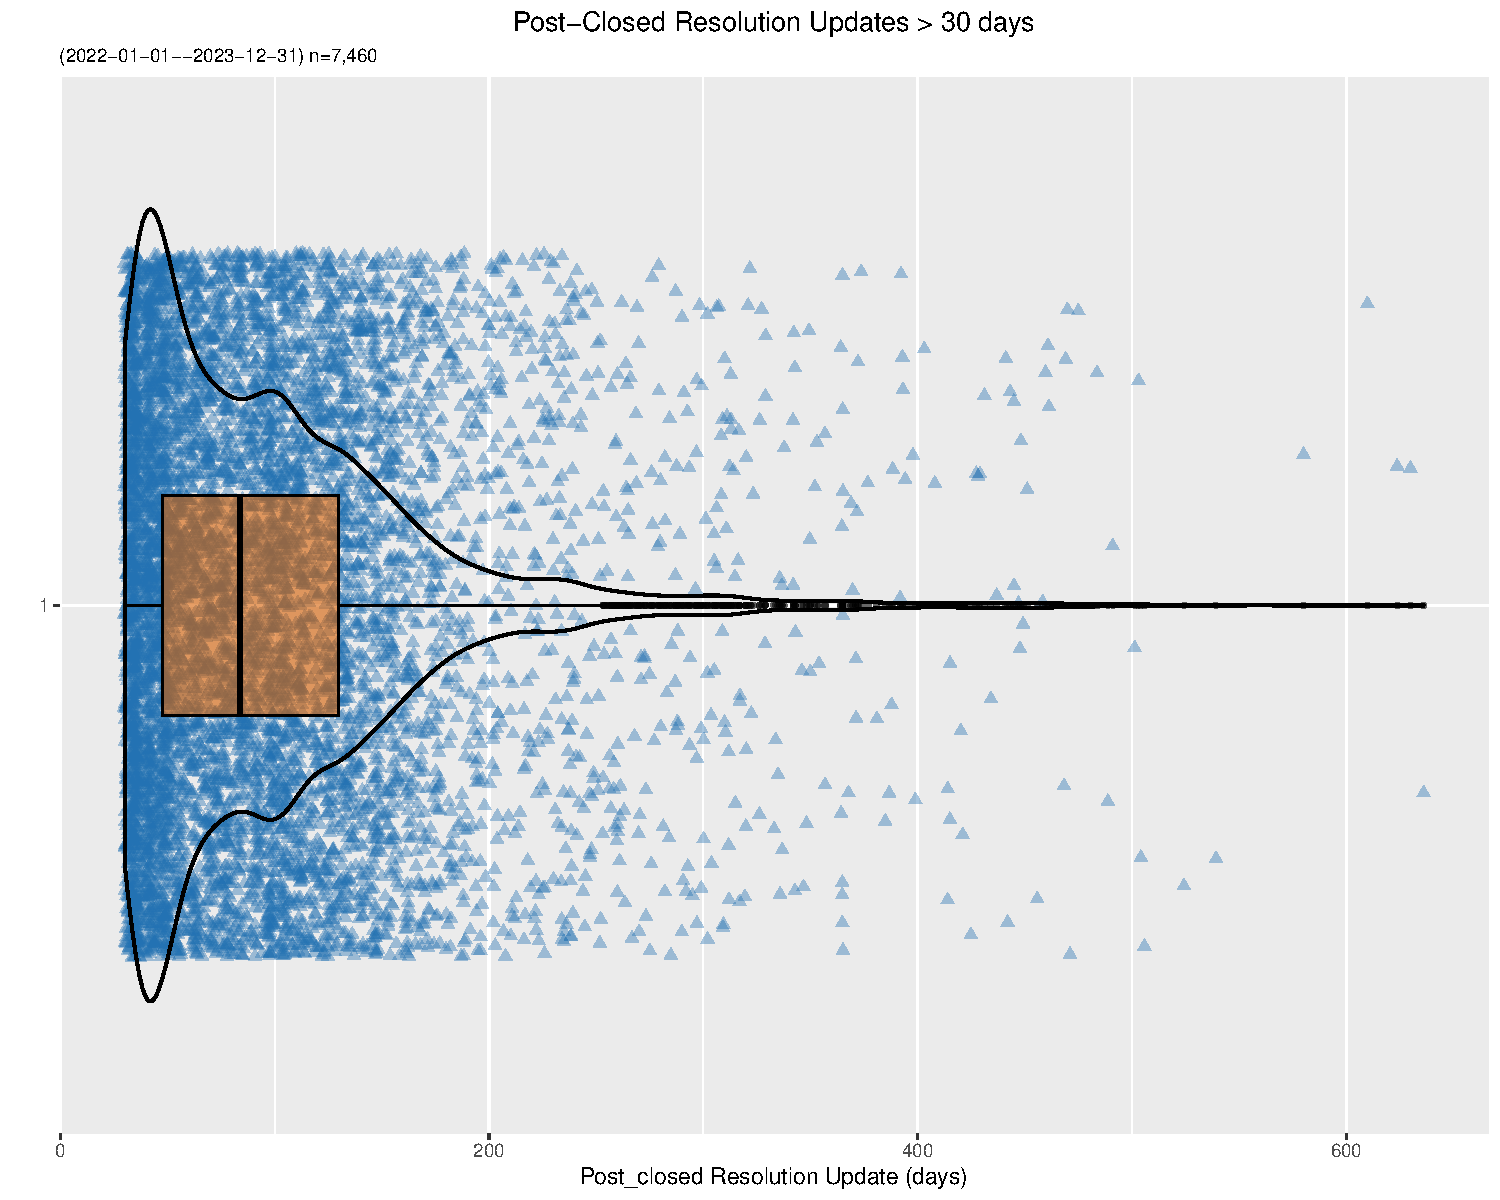
\includegraphics[width = 0.7\textwidth]{post_closed_violin_chart.pdf}
  \caption{Post-closed resolution action update date(s) over 30 days.}
  \label{fig:resolution-violin}
\end{figure}

\jy{Are these from 2-year or 10-year period? Need to clarify in
  Section 2.}

A similar issue occurs when resolution action update date is after the
closing date. \jy{It might be possible, I think, if they allow updates
  after a SR is closed.}
When an SR is updated, the 311 software automatically populates the 
\texttt{resolution\_action\_update\_date}. Some of these updates 
occur long after the SR is closed. As shown in Figure~\ref{fig:resolution-violin}, 
there are 7,460 SRs that were updated more than 30 days after the 
\texttt{closed\_date}, but less than 730 days, to exclude infeasible 
dates like 1900-01-01. The chart highlights the distribution of these 
post-closure updates, with a notable concentration of updates within 
the 30-to-90-day range. This pattern raises questions about whether 
such delayed updates are standard operational practice or indicative 
of a potential issue requiring further investigation. While the reason 
for these delayed updates is unclear, they may impact the accuracy of 
response time analyses if not properly accounted for.
	
\subparagraph{Same Created Date \& Closed Date: Zero Durations}
A more prevalent issue occurs when the \texttt{closed\_date} and 
\texttt{created\_date} are exactly the same, down to the second. This 
creates a \textbf{zero duration}, which is also nonsensical. There 
are 191,141 such SRs, representing 3.1\% of all non-blank data. 
Ninety-nine percent of these zero-duration SRs occur in five agencies:
DHMH, DOT, DOB, DSNY, and DEP.. 
This distribution does not mirror the overall SR distribution by 
agency, suggesting an agency-specific issue.
	
		
%\begin{figure}[tbp]
%	 \centering
%	 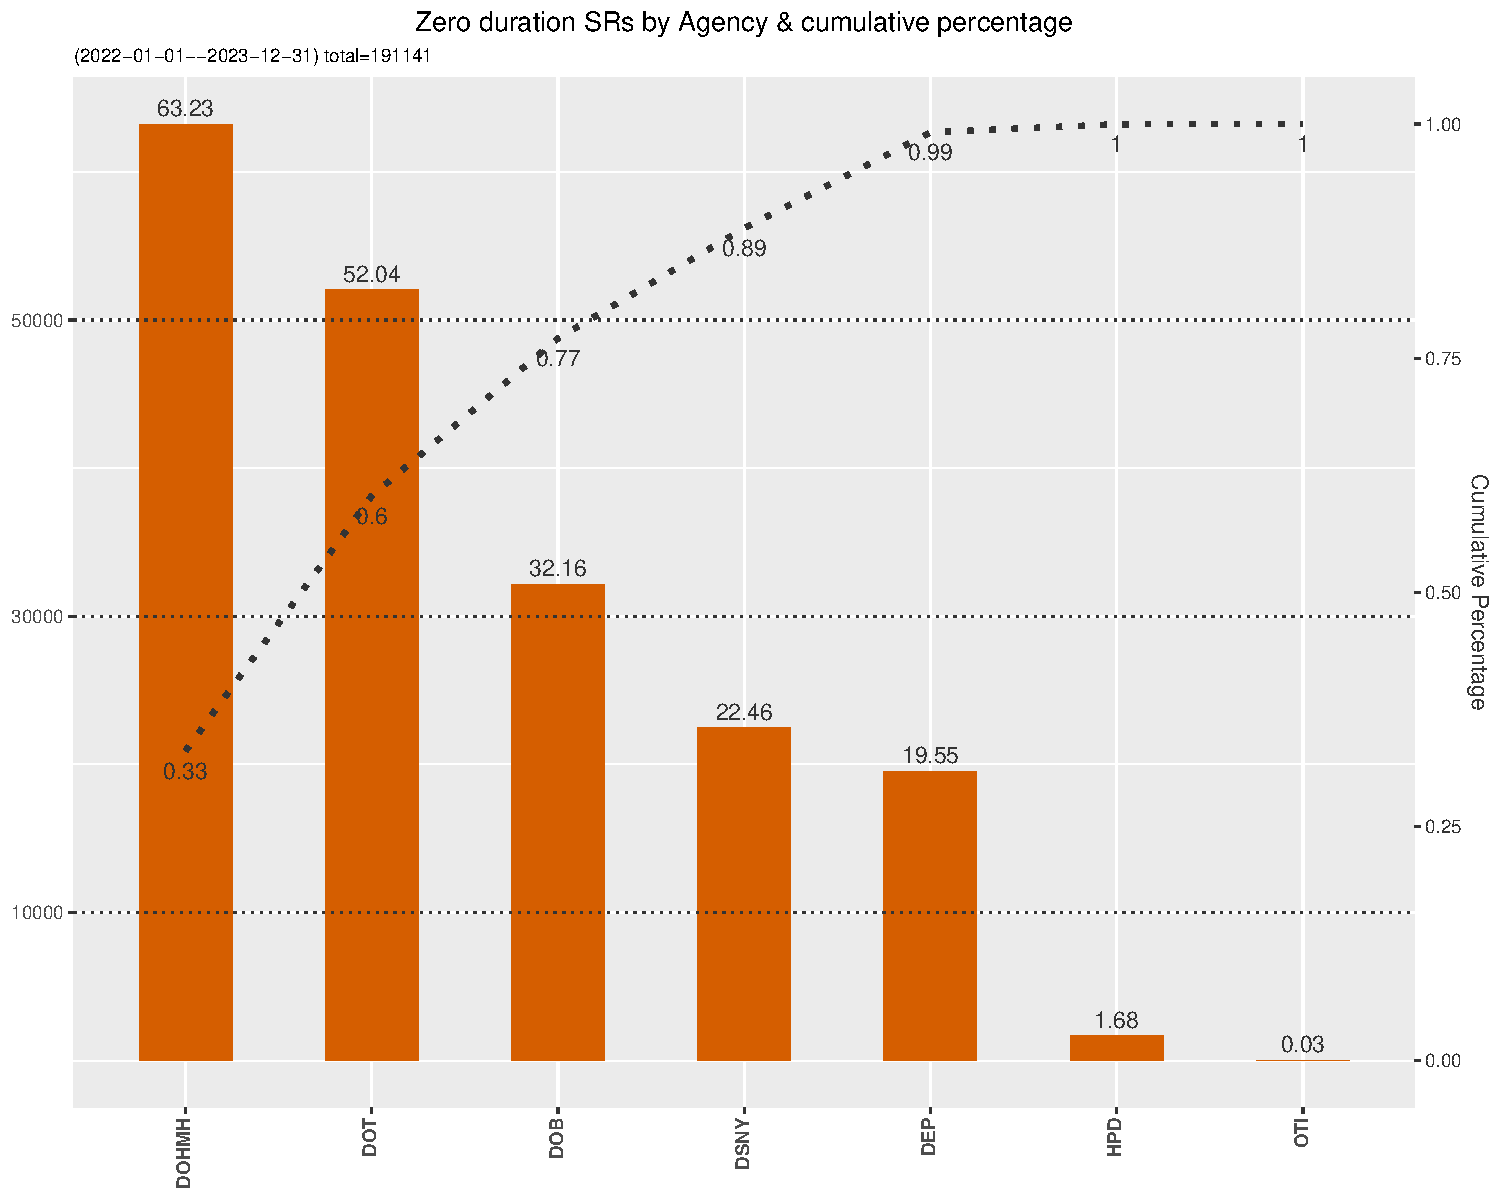
\includegraphics[width = \textwidth]{zero_duration_SR.pdf}
%	 \caption{SRs with Zero Durations by Agency}
%	 \label{fig:zero-duration}
%\end{figure}	

\subparagraph{Created Date or Closed Date(s) at Midnight or Noon}
Another issue found with the \texttt{created\_date} and 
\texttt{closed\_date} fields is the unusually large number of SRs 
created or closed at exactly midnight (00:00:00) or noon (12:00:00), 
down to the second. Normally, SR creation and closure follow the 
work-day schedule, with most SRs created during daylight hours and 
fewer at night or in the early morning. However, there is a 
significantly higher number of SRs closed exactly at midnight and noon, 
as well as a large number created exactly at noon. Specific observations 
include:
\begin{itemize}
    \item 99,779 SRs were created exactly at noon (12:00:00).
    \item 235,347 SRs were closed exactly at midnight (00:00:00).
    \item 105,505 SRs were closed exactly at noon.
\end{itemize}


\begin{figure}[tbp]
  \centering
  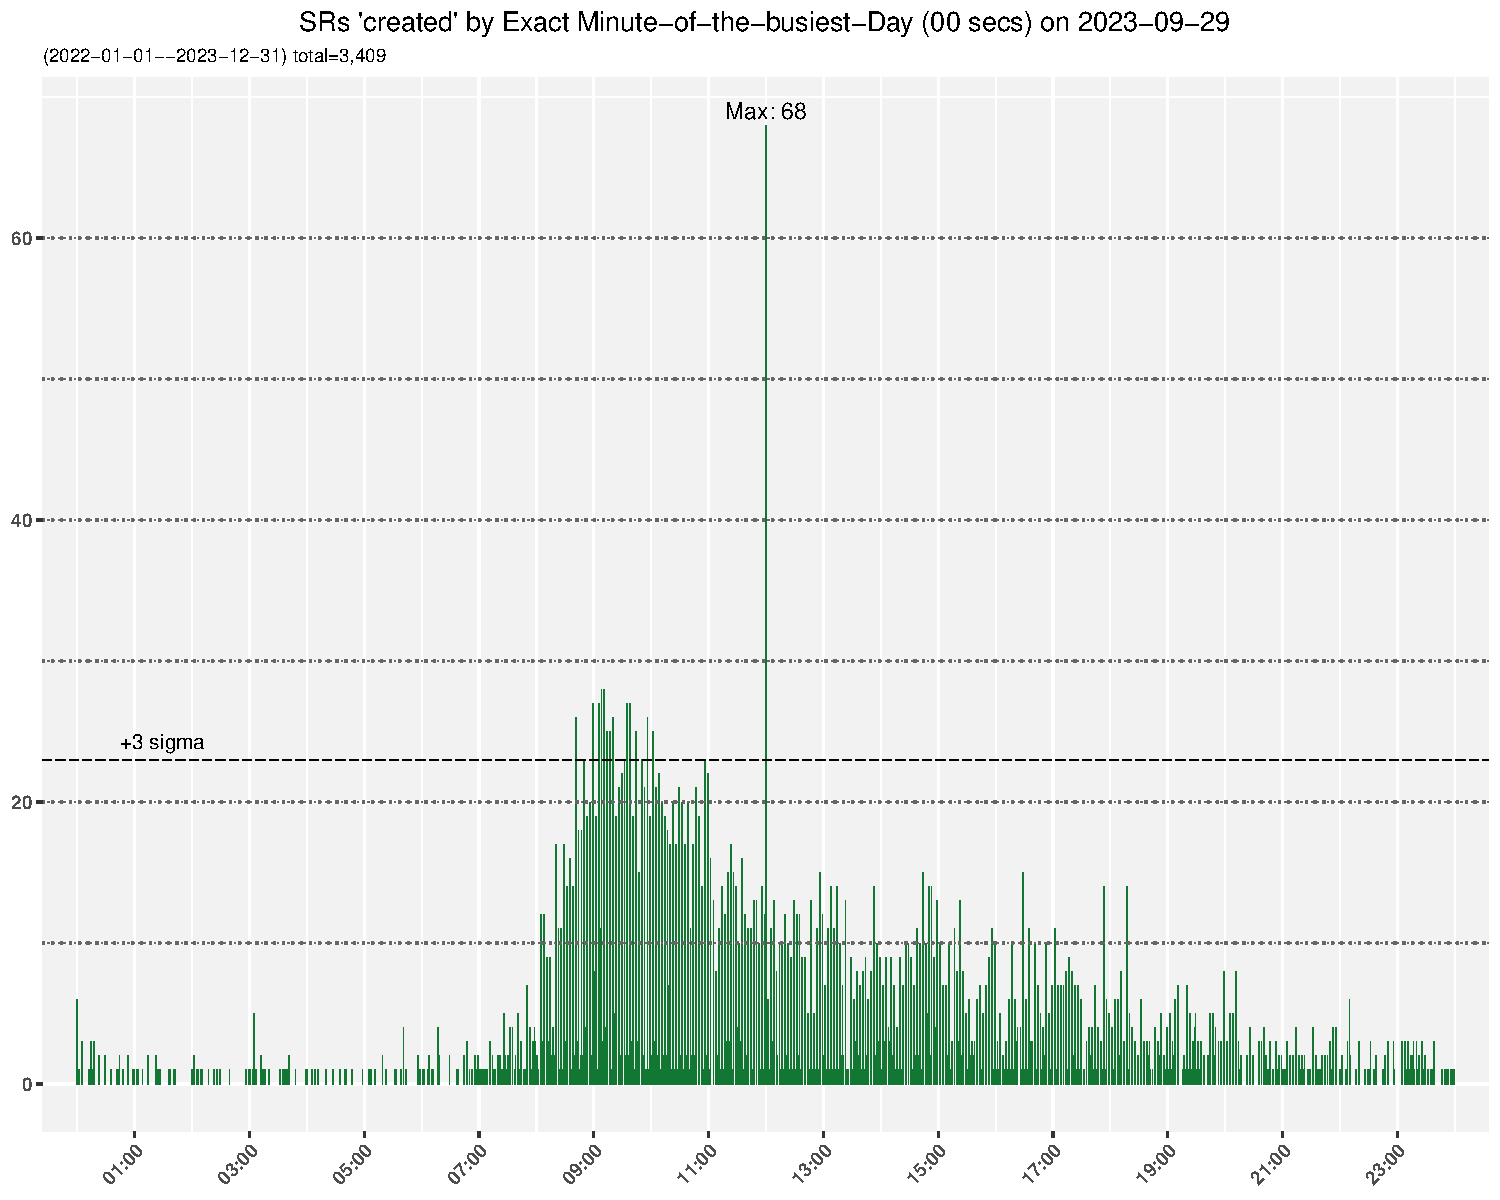
\includegraphics[width=0.7\textwidth]{2-year-trend_SR_created_by_minute_of_busiest_day.pdf}
  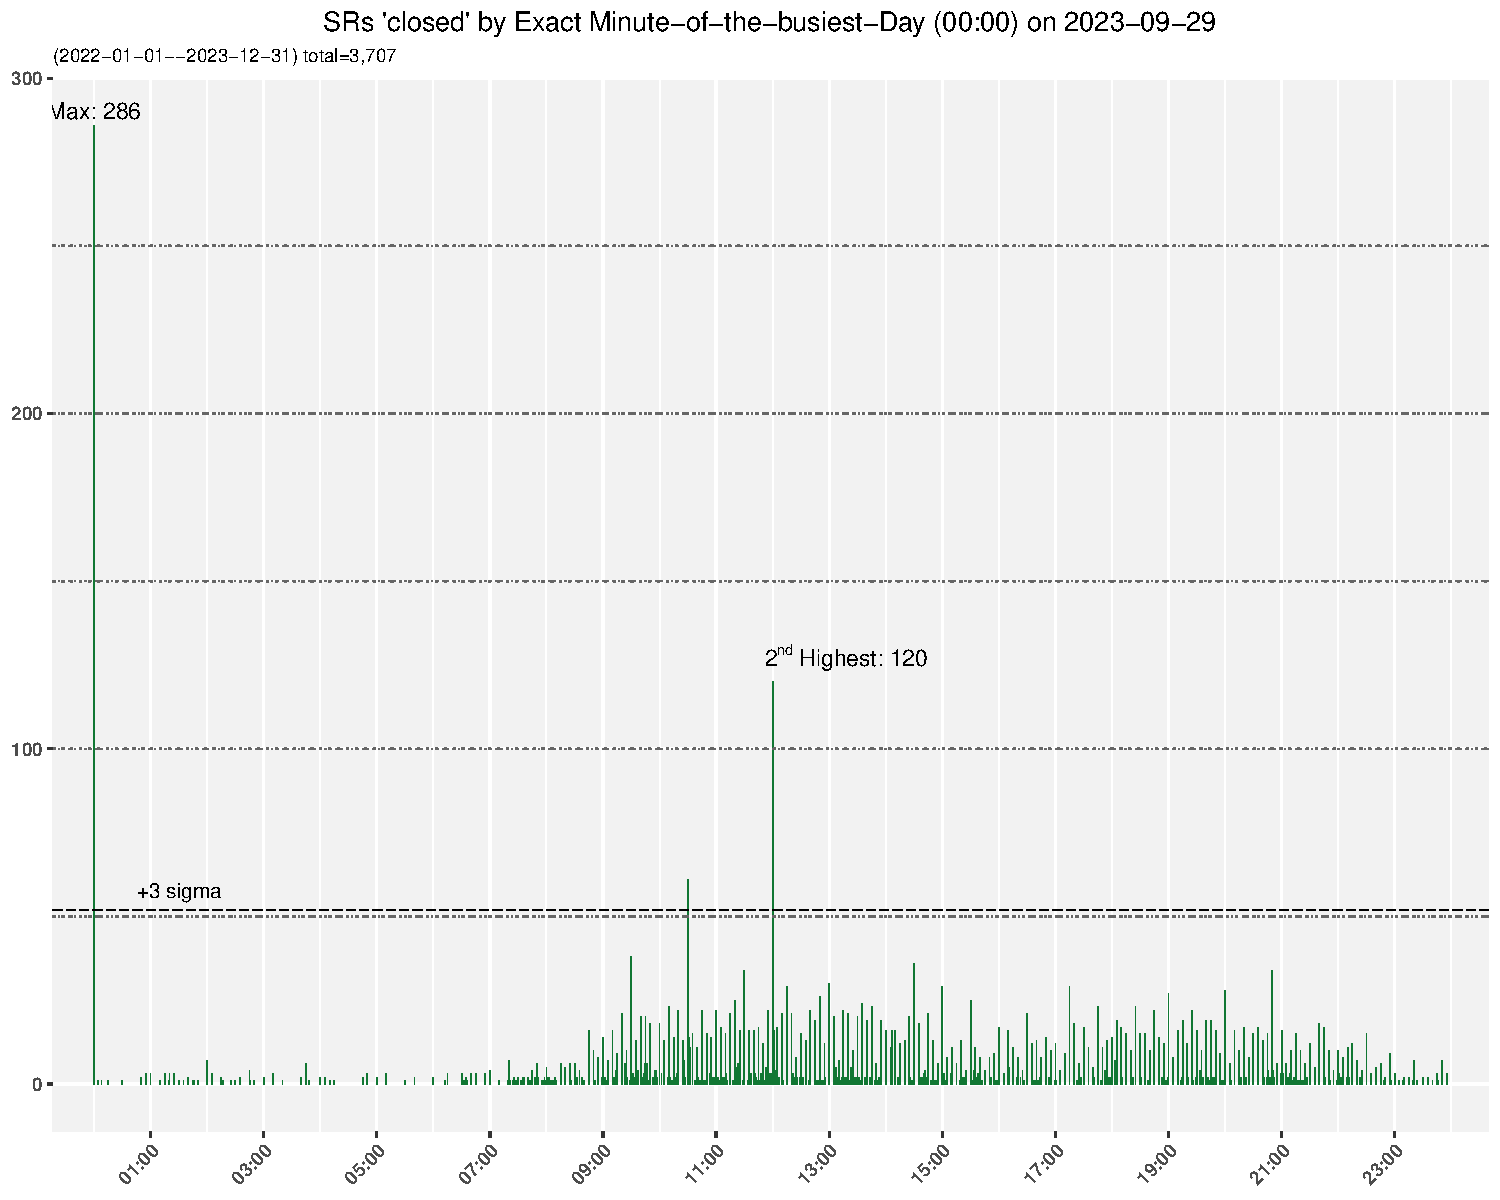
\includegraphics[width=0.7\textwidth]{2-year-trend-SR_closed_by_minute_of_busiest_day.pdf}
  \caption{SRs Created and closed minute-by-minute on busiest day
    during two year period \jy{give years}.}
  \label{fig:busiest}
\end{figure}	

Figure~\ref{fig:busiest} visualizes this anomaly by examining the 
busiest day during this 2-year period (Friday, 2023-09-29). The 
\texttt{created\_date} values are aggregated by minute (with seconds 
equal to zero), providing a minute-by-minute look at SR creation on 
that day. Notably, there is a spike exactly at noon (12:00), well 
beyond the 3\textsigma{} line. \jy{May not want to mention 3 sigma as
  here we have highly skewed count data.}
The same analysis was repeated for 
\texttt{closed\_date} values on the busiest day, aggregated by minute 
(with seconds equal to zero). Spikes were observed at both 00:00:00 
and 12:00:00.


These unusual patterns of SR creation and closure exactly at midnight 
and noon suggest the presence of a bulk create/close software process 
that automatically assigns time stamps of midnight (00:00:00) or noon 
(12:00:00) to large batches of SRs. This behavior distorts the 
calculated duration of these SRs by providing inaccurate dates. The 
distribution by agency shows that over 90\% of the ``created-at-noon'' 
SRs come from just two agencies: DOB and DSNY. Further investigation 
reveals that a single agency, DSNY, is responsible for over 99\% of 
the ``closed-at-noon'' SRs.



	
\subsection{Accuracy and precision}
\label{sec:precision}

\jy{This is caused by reading the number in as double
  precision. Single precision would be good.}


An question of precision vs. accuracy arises with the Latitude 
and Longitude fields. Both Latitude are expressed as 
a 14-decimal number, e.g. 40.86769186022511. Given 
that 1 degree of latitude at the equator is equal to 111.044736 
kilometers, the ``1'' at the end of that number represents 
approximately 1.1 nanometers (1/1,000,000,000 of a meter). For 
reference a DNA molecule is approximately 2nm in width. Clearly 
the representation of the Latitude and Longitude fields is a 
classic case of 14-digit precision, but limited accuracy. 



\subsection{Redundant \& Duplicate fields}
\label{sec:duplicates}

During this analysis, several redundant fields were observed and should 
be examined for possible consolidation.

\textbf{Latitude/Longitude and Location:} The \texttt{location} field 
is a pure concatenation of the latitude and longitude fields with a 
comma and parentheses added. This makes the \texttt{location} field 
arguably harder to use than the individual fields. For example:  
\texttt{latitude}: 40.768456429488, \texttt{longitude}: $-$73.9575661888774, 
and \texttt{location}: (40.768456429488, $-$73.95756618887745).

\textbf{borough \& park\_borough:} These two fields are fully redundant, 
as they are 100\% matches.

\textbf{borough \& borough\_boundaries:} These fields are 98.3\% matches. 
This ``near-duplicate'' relationship creates a challenge in determining 
which field is correct when discrepancies arise.

\textbf{borough \& taxi\_company\_borough:} Despite their names, these 
fields are almost entirely different, with only a 0.05\% match. The 
\texttt{taxi\_company\_borough} field is used exclusively by the TLC, 
indicating a need for consultation with TLC to understand the differing 
uses.

\textbf{incident\_zip \& zip\_codes:} The \texttt{zip\_codes} field, 
one of the computed fields, was found to have 56\% invalid entries, 
while the \texttt{incident\_zip} field has a 99.93\% accuracy rate. 
We recommend eliminating or masking the \texttt{zip\_codes} field 
until its accuracy can be improved.

\textbf{police\_precinct \& police\_precincts:} These two computed 
fields are 99.9\% matches. Since the computational process is unknown, 
it is unclear which field is more accurate. However, having two fields 
with near-duplicity suggests that only one is necessary.

\textbf{agency \& agency\_name:} The \texttt{agency} field contains 
abbreviations of City agencies (e.g., NYPD, DOT), while 
\texttt{agency\_name} contains the full names. Including both seems 
redundant, especially given the space taken up by full names in the 
CSV file.

\textbf{landmark \& street\_name:} While the \texttt{landmark} field is 
intended for noteworthy locations (e.g., parks, airports), most entries 
are actually street names, with a 62\% match to \texttt{street\_name}. 
Even non-matches (excluding blanks) appear to be similar, differing 
only in spelling or formatting (e.g., ``NINTH AVE'' vs. ``9 AVE''). This 
indicates a possible misuse of the \texttt{landmark} field.

\textbf{cross\_street\_1 \& intersection\_street\_1 and cross\_street\_2 
\& intersection\_street\_2:} These two sets of street pairs are used to 
help identify the incident address. After applying address 
standardization using the R \textit{campfin} package, we found 88\% of 
these pairs to be duplicates, while 12\% do not match. This discrepancy 
raises the question of which field should be trusted. It is possible 
that the two pairs originated from different agencies that used 
different variable names to represent the same information, but no 
documentation exists to clarify this relationship.

\paragraph{Near Match}

\jy{This investigation could be relegated to on online supplement
  given the low percentage of near-match. It's taking too much spaces
  here.
}

\begin{table}[tbp]
    \centering
     \caption{Examples of near-matches for cross\_street\_1 and intersection\_street\_1.}
     \label{tab:x1nearmatches}
		\begin{tabular}{l l l r}
	        \toprule
	        \textbf{cross\_street\_1} & \textbf{intersection\_street\_1} 
	        & \textbf{agency} & \textbf{hamming\_distance} \\
	        \midrule
	        WEST 168 ST    & WEST 167 ST           & DOT    & 1 \\
	        105 AVE        & 107 AVE               & DOT    & 1 \\
	        145 ST         & 150 ST                & DOT    & 2 \\
	        138 ST         & 139 ST                & DOT    & 1 \\
	        19 AVE         & 20 AVE                & DOT    & 2 \\
	        76 ST          & 79 ST                 & DOT    & 1 \\
	        67 ST          & 68 ST                 & DOT    & 1 \\
	        \bottomrule
	    \end{tabular}
\end{table}

\begin{table}[tbp]
    \centering
    \caption{Summary of cross\_street\_1 and intersection\_street\_1}
    \label{tab:summary1}
	    \begin{tabular}{l r r}
	        \toprule
	        \textbf{category} & \textbf{count} & \textbf{percentage} \\
	        \midrule
	        Matching                    & 5,637,182 & 88.15     \\
	        Both blank -- Matching      & 1,624,499 & 25.4      \\
	        Non-matching                &   757,726 & 11.85     \\
	        cross\_street\_1\_blank     &   222,232 & N/A       \\
	        intersection\_street\_1\_blank &   519,348 & N/A       \\
	        Near-match                  &       128 & 0.002002  \\
	        \bottomrule
	    \end{tabular}
\end{table}

In addition to the matching values, we encountered a number of 
\textit{near-matches}, situations where the \texttt{cross\_street} 
and \texttt{intersection\_street} are nearly, but not exactly, identical. 
An example of such a near-match is when one field reads ``HARMON DR'' 
and the other reads ``HARMON RD.'' To identify these near-matches, 
we applied the \href{https://en.wikipedia.org/wiki/Hamming_distance}
{\textit{Hamming Distance}}, which measures the number of character
\jy{needs a quick definition and reference}
changes required to make the two fields identical. For this analysis, 
we set the threshold for a near-match to a Hamming Distance of two (2).


Table~\ref{tab:x1nearmatches} provides examples of near-matches for 
\texttt{cross\_street\_1} and \texttt{intersection\_street\_1}. These 
entries show slight variations in the street name or number, such as 
``WEST 168 ST'' and ``WEST 167 ST,'' both processed by DOT, where only 
one character differs. Although these discrepancies may seem small, 
they can have implications for data accuracy, particularly when 
geocoding or matching locations for analysis purposes.


Table~\ref{tab:summary1} presents a summary of the match and 
near-match results for \texttt{cross\_street\_1} and 
\texttt{intersection\_street\_1}. As the table shows, 88.15\% of the 
entries are exact matches, while 25.4\% are blank but matching. 
However, 11.85\% of the entries are non-matching, and a small fraction 
(0.002\%) fall into the near-match category. Although this percentage 
seems negligible, even a small number of near-matches can lead to 
confusion or errors when analyzing location-based data, especially 
if critical decisions rely on accurate street data. Address 
standardization or correction processes may be necessary to resolve 
these inconsistencies and improve the reliability of the data.


\subsection{Storage}
\label{sec:filesize}

By removing duplicate and ``near-duplicate'' fields, it is possible to 
shrink the file size by 12.3\%, which for this large dataset equates to 
a reduction of 395 Mb. A smaller file size means faster downloads, 
less storage impact, and simpler data analysis efforts.
Below is a list of duplicate and near-duplicate fields. There are 
challenges with these proposed deletions, especially with the 
``near-duplicate'' fields. For example, while the \texttt{park\_borough} 
is a complete duplicate of the \texttt{borough} field, the 
\texttt{borough\_boundary} field is only 98.3\% similar. Although losing 
1.7\% of the data is small, it still amounts to 110,715 non-matching 
occurrences. The authors propose deleting the following fields:

\begin{itemize}
    \item \textbf{agency\_name}: Each row contains the \texttt{agency} field, 
    which uses abbreviations that are clear and well understood.
    
    \item \textbf{park\_borough}: A 100\% match with the \texttt{borough} field, 
    leading to no data loss.
    
    \item \textbf{location}: A straight concatenation of latitude and longitude 
    fields, offering no additional value beyond duplication.
    
    \item \textbf{police\_precinct}: This field has a 99.95\% match with 
    \texttt{police\_precincts}. Removing one would result in minimal data loss.
    
    \item \textbf{borough\_boundaries (computed field)}: A 98.3\% match 
    with the \texttt{borough} field.
    
    \item \textbf{cross\_street\_1 \& 2 and intersection\_street\_1 \& 2}: 
    An 88\% match between these pairs. We recommend deleting the 
    \texttt{intersection\_street\_1 \& 2} fields while acknowledging some 
    data loss.
    
  \item \textbf{zip\_codes (computed field)}:
    This field has a 58\% error rate and can lead to significant 
    analytical errors. We recommend deleting this field.
\end{itemize}

Additionally, certain fields may not be useful due to their sparse population. 
For example, the \texttt{taxi\_company\_borough} field is 99.94\% blank, 
\texttt{road\_ramp} is 99.8\% blank, \texttt{vehicle\_type} is 99.7\% blank, 
and \texttt{due\_date} is 99.6\% blank. Several other fields, such as 
\texttt{bridge\_highway\_direction}, \texttt{bridge\_highway\_name}, 
\texttt{bridge\_highway\_segment}, and \texttt{taxi\_pick\_up\_location}, 
are over 99\% blank, with most used exclusively by the TLC.


Further reduction is possible by coding categorical 
variables, such as \texttt{complaint\_type}, through methods like dropdown 
menus or encoded categories. By using a dropdown menu for 
\texttt{complaint\_type}, data entry can be standardized, reducing 
inconsistencies caused by manual input errors. Additionally, categorical 
variables with a limited set of possible values can be stored more 
efficiently by assigning unique codes or numerical representations for 
each category. For instance, instead of repeatedly storing the full text 
for every complaint type (e.g., ``Noise - Residential,'' ``Noise - 
Commercial''), a single code could represent each type. This not only 
reduces file size but also improves data processing speed and efficiency 
during analysis. Moreover, standardizing categorical inputs prevents 
the inclusion of misspellings or unrecognized entries, ensuring cleaner 
and more reliable data. This approach is particularly useful in large 
datasets, where frequently repeated categorical variables can 
significantly increase storage requirements. Encoding such fields 
as dropdown options or coded variables can lead to faster query times 
and more consistent data handling.



\subsection{Data Dictionary} 
\label{sec:datadictionary}

The Data Dictionary could benefit from an update. We found several 
discrepancies between the Data Dictionary and the actual data, which 
could potentially mislead analytic efforts.

\begin{itemize}
    \item While the Open Data portal lists the data types of various 
    fields, the Data Dictionary does not. Nor does it provide details 
    on specific fields, such as constraints or the domain of legal 
    values. For example, the \texttt{incident\_zip} field is specified 
    as ``text.'' This may not be the most suitable definition; 
    ``categorical,'' with a note that the data contains only numeric 
    characters and is not subjected to arithmetic operations, might 
    be a better description.
    
    \item Many of the domains of legal values are incomplete or 
    inaccurate. For example, the Data Dictionary indicates that the 
    \texttt{status} field has values of \textit{assigned, canceled, 
    closed}, or \textit{pending}, but we also found values such as 
    \textit{in progress, started}, and \textit{unspecified}. 
    Additionally, no SRs were found with a status of 
    \textit{canceled}. The \texttt{address\_type} field similarly 
    lists values of \textit{address, blockface, intersection, latlong}, 
    and \textit{placename}, but we found additional values such as 
    \textit{bbl} and \textit{unrecognized}, and no \textit{latlong} 
    values were observed. Other fields, like \texttt{facility\_type}, 
    \texttt{vehicle\_type}, \texttt{taxi\_pick\_up\_location}, 
    \texttt{road\_ramp}, and \texttt{city}, exhibit similar inaccuracies 
    in their specified domain values.
    
  \item As mentioned earlier, six \texttt{@computed} fields that are
    present in the data but not included in the Data Dictionary need
    to be documented.
\end{itemize}


\section{Government Open Data Curation Recommendations}
\label{sec:recommendations}
Building upon the insights gained from our case study of the 
NYC 311 Service Request (SR) data, we propose a set of data 
curation principles tailored for government-released open datasets. 
These principles are designed to address the unique challenges 
and requirements observed in the curation of such datasets, 
ensuring that they remain reliable, consistent, and useful for 
public services, research, and other applications.

\subsection{Principles}
\paragraph{Principle 1: Ensuring Consistency Across Agencies and Time}
A key challenge in government-released datasets is the 
harmonization of data fields across various agencies and 
maintaining this consistency over time. As seen in the NYC 
311 data, discrepancies in field names, formats, and definitions, 
such as those between \texttt{police\_precinct} and 
\texttt{police\_precincts}, can introduce significant 
inconsistencies. To address this, agencies should adopt 
standardized naming conventions and formats across all datasets. 
Regular audits and data harmonization processes should be 
implemented to ensure consistency across long-term datasets, 
particularly as agency structures or reporting standards evolve. 
For instance, ensuring that historical datasets reflect the same 
field naming conventions over a span of years can prevent 
inconsistent analyses.

\paragraph{Principle 2: Guaranteeing Accuracy and Validity in Data Entry}
Data accuracy and validity are fundamental to the utility of 
open datasets. In the NYC 311 data, issues such as 
invalid zip codes (e.g., 58\% invalid \texttt{zip\_codes} entries) and 
nonsensical date entries (e.g., negative durations) highlight the need 
for rigorous validation processes. Governments should establish 
clear protocols for data entry, ensuring that fields are populated with 
valid, legally acceptable values. For example, fields like 
\texttt{created\_date} and \texttt{closed\_date} should be subject to 
automated checks that prevent logical errors, such as closing an 
SR before it was opened. Ensuring the integrity of critical fields 
like geographic locations and agency names enhances the quality 
and reliability of the data.

\paragraph{Principle 3: Optimizing Storage and Representation Efficiency}
Efficient storage and data representation are crucial for handling 
large government datasets. By eliminating redundant fields and 
encoding categorical variables, agencies can significantly reduce 
file sizes and improve the efficiency of data analysis. In the NYC 
311 dataset, for example, redundant fields such as \texttt{borough} 
and \texttt{park\_borough} could be consolidated without any data 
loss, saving space and reducing file size by up to 12.3\%. Another 
example is the \texttt{taxi\_company\_borough} field, which is 99.94\% 
blank and should be evaluated to determine if its inclusion is 
necessary. Similarly, categorical variables like \texttt{complaint\_type} 
could be encoded in a standardized format to optimize storage and 
streamline analyses. Reducing file size not only saves storage space 
but also enhances the performance of queries and analysis processes.

\paragraph{Principle 4: Updating Data Dictionaries and Documentation}
Clear and accurate documentation is essential for the effective use 
of government-released datasets. The NYC 311 data revealed several 
issues where the Data Dictionary did not accurately reflect the 
actual data, such as missing field descriptions for computed fields. 
Updating the Data Dictionary to include descriptions of all fields, 
especially computed fields like \texttt{@computed\_region\_xxxx}, 
would improve transparency and usability. Regular updates should 
be made to ensure that any changes in data structure or content are 
reflected. This practice enhances the ability of external users, 
including researchers and developers, to understand and work 
effectively with the data.

\paragraph{Principle 5: Automating Quality Assurance Processes}
Automating data validation and quality assurance processes can 
significantly improve the reliability of government datasets. In the 
NYC 311 case, issues such as large spikes in SR creation and closure 
at exactly midnight or noon likely stem from automated processes that 
distort the accurate capture of SR durations. By implementing 
real-time validation tools, governments can prevent such anomalies 
from entering the dataset. Automated systems can be designed to 
flag inconsistencies, incorrect values, or illogical sequences, such 
as invalid \texttt{incident\_zip} values or illogical date entries. 
Automation can also facilitate faster detection and correction of 
errors, reducing the need for manual intervention and ensuring 
the data remains clean and reliable as it is continuously updated.

\paragraph{Principle 6: Addressing Data Transparency and Accessibility}
Transparency is a core tenet of open data, and governments must ensure 
that datasets are not only accurate but also accessible and easily 
understandable. This involves providing clear metadata and making 
datasets available in user-friendly formats. For example, in the NYC 
311 dataset, fields like \texttt{@computed\_region\_xxxx\_xxxx} and 
the distinction between \texttt{incident\_zip} and \texttt{zip\_codes} 
can be confusing for non-expert users. These fields should be clearly 
documented, explaining how they are calculated and how they differ. 
Additionally, governments should communicate transparently about 
data quality issues, such as notifying the public when errors in SR 
fields (e.g., erroneous closed dates) are discovered and explaining 
how such issues will be resolved. By ensuring transparency and 
keeping the public informed, governments foster trust and promote 
wider use of datasets for research, civic engagement, and innovation.


\subsection{Actionable Steps}
While these principles are broad, actionable steps are required to 
implement them effectively. Governments can begin by investing in 
real-time validation systems, regular updates to data dictionaries, 
and tools for encoding and standardizing data fields. For example, 
systems that automate the enforcement of data validation rules 
(e.g., flagging incorrect zip codes) can significantly improve data 
quality. Collaboration with city agencies and stakeholders is crucial 
to ensure that data standards, formats, and metadata meet the needs 
of diverse users, including policymakers, researchers, and the 
general public. Regular communication between agencies and external 
users can help identify recurring issues and areas where improvements 
are needed. By facilitating regular communication and collaboration 
with various stakeholders, governments can ensure data remains relevant 
and actionable for public use.


Engagement with data scientists and statisticians is key to improving 
data curation strategies. These experts can help design and refine 
curation processes, such as creating algorithms for automatic data 
cleaning, identifying inconsistent data entries, and ensuring the 
dataset’s structure is maintained over time. Their expertise is also 
critical in developing protocols for validating incoming data, correcting 
errors in real-time, and ensuring consistency across multiple data sources. 
Feedback from statisticians and data scientists, such as the issues reported 
in this paper, needs a clear and accessible channel to reach the 311 SR data 
team and other relevant city agencies. Establishing such feedback loops 
ensures that recommendations for improving data curation and validation 
are not only heard but implemented. This feedback mechanism would also allow 
ongoing dialogue between data users and city officials, leading to more dynamic 
and responsive data management practices.


A particularly valuable avenue for engagement is through events such as NYC 
Open Data Week, which fosters collaboration and innovation across sectors. 
Our involvement in this project stemmed from such an event, where we were 
inspired by the potential of open data to enhance public services. Governments 
should continue supporting these kinds of initiatives, which not only promote 
data literacy but also encourage community-driven improvements to datasets. 
By leveraging the expertise of data scientists, statisticians, stakeholders, 
and civic organizations, governments can ensure that their open datasets 
remain accurate, transparent, and useful for a wide range of applications.


% \begin{itemize}
% \item  Undertake a dedicated effort 
%     to investigate these data anomalies, confirm the veracity of the 
%     issues, and collaborate with the appropriate Agency Open Data 
%     Representatives to find resolutions. This effort may be complex 
%     and require software changes. Coordination and mutual approval 
%     of changes will be key, requiring strong support from senior 
%     leadership.

%     \item Standards and protocols should be established, agreed upon, 
%     and enforced. This includes defining the domain of legal values, 
%     ensuring data accuracy, implementing address normalization, 
%     clarifying data usage, and providing detailed data definitions.

%     \item Resolve many potential data integrity issues
%     through enforcement by software. For instance, software should 
%     prevent invalid entries like erroneous zip codes. Similarly, fields 
%     like \texttt{created\_date} and \texttt{closed\_date}, which 
%     measure responsiveness, should have logic checks to prevent 
%     illogical sequences, such as an SR being ``closed'' before 
%     being ``opened.''

%     \item The large spikes in SR creation and closure at midnight and 
%     noon likely point to automated processes from external Agency 
%     integrations. These distortions should be eliminated in favor of 
%     capturing accurate SR durations with precise timestamps.

%     \item As discussed, there are six ``computed'' fields that are not 
%     listed in the Data Dictionary. Some of these fields contain 
%     significant inaccuracies. We recommend updating the Data 
%     Dictionary and, if necessary, masking these fields from public use 
%     until their accuracy is improved.

%     \item Duplicate fields should be reviewed for removal. In some 
%     cases, such as \texttt{borough} and \texttt{park\_borough}, the 
%     duplication is 100\%. In others, the match is 80-90\%. 
%     These near-duplicates should be assessed to determine their 
%     relevance in the 311 SR dataset. Initial analysis suggests that 
%     removing these fields could reduce file size by up to 12\%, with 
%     further reductions possible upon deeper review.

%     \item Fields with very low data presence, such as 
%     \texttt{taxi\_company\_borough}, populated only 0.06\% of the time, 
%     should be evaluated to determine if they are necessary.

%     \item The Data Dictionary, last updated in March 2023, should be 
%     revised based on the issues discussed in Section~\ref{sec:datadictionary}.

%     \item The precision of latitude, longitude, and location fields 
%     should be reduced. We recommend limiting precision to four 
%     decimal places (0.000X), which represents approximately 36.4 feet. 
%     More decimal points strain credibility.

%     \item The 11 address-related fields (\texttt{incident\_address}, 
%     \texttt{street\_name}, \texttt{city}, \texttt{intersection\_street\_1 \& 2}, 
%     \texttt{cross\_street\_1 \& 2}, \texttt{landmark}, \texttt{road\_ramp}, 
%     \texttt{bridge\_highway\_segment}, and \texttt{taxi\_pick\_up\_location}) 
%     should be standardized to USPS format. Software can easily 
%     perform this standardization.

%     \item There are multiple ways missing data is represented, such as 
%     ``UNKNOWN'', ``N/A'', ``NA'', ``na'', and blanks (`` ''). Protocols 
%     should be established to standardize the representation of missing data.
% \end{itemize}

\section{Discussion} \label{sec:discussion}

Our study highlights the critical role of robust data curation in
ensuring the reliability and utility of open datasets, as demonstrated
through the examination of the NYC 311 data. As these datasets are
applied across diverse fields such as public services and academic
research, inconsistencies, missing values, and formatting errors can
significantly undermine the insights derived from them. Trustworthy
machine learning systems, which rely heavily on high-quality data, are
especially vulnerable to such issues. Errors in the underlying data,
such as biases or inconsistencies, can compromise both the accuracy
and fairness of predictive models, impacting real-world decisions in
urban planning and policy \citep{rahm2000data, geiger2020garbage}.


This research further emphasizes the necessity of harmonizing data
across city agencies, particularly in resolving discrepancies in field
names, formats, and definitions. Consistency in data is essential for
trustworthy machine learning, where inconsistencies across sources can
lead to distorted outcomes. This challenge is even more pronounced in
datasets that span long time periods, as changes in agency structures
or reporting standards can introduce subtle biases. Long-term data
consistency is crucial for longitudinal studies and predictive
modeling, as even minor data shifts can lead to significant deviations
in model outcomes, as noted by \citet{rahm2000data} and
\citet{borgman2012conundrum}.


Finally, the intersection of data curation and machine learning for
public policy applications opens new avenues for improving governance.
High-quality data enables machine learning models to better predict
trends, allocate resources, and address service delivery issues, such
as delays in responding to 311 complaints. The COVID-19 pandemic
underscored the importance of real-time, trustworthy data in crisis
management, where the accuracy and timeliness of data-driven insights
were critical for public health responses. Without proper data
curation, machine learning models used during the pandemic would have
been compromised, affecting decisions on resource allocation and
service provision \citep{worby2020face, khemasuwan2021applications}.
Future efforts could focus on automating data curation processes,
particularly in real-time data pipelines, to ensure that the data used
in machine learning models remains accurate, clean, and reliable
\citep{chu2016data, hurbean2021open}.


\section*{Supplementary Material}
The NYC 311 SR data and code used to produce the results reportred in
this paper are available [FixMe].
\jy{need to think: we need to keep a copy of the downloaded data;
  if the data portal changes and our code may not work.}



\bibliographystyle{jds}
\bibliography{refs}

\end{document}